% =====================================================================
%  NeuroFly-Bee Perú — Artículo IEEE (máx. 12 páginas)
%  MIA-203 Redes Neuronales y Aprendizaje Profundo — UNI FIIS
%  Desde v18 cada sección vive en secciones/ y tiene un dueño (ver CODEOWNERS):
%  así cinco personas escriben a la vez sin conflictos de merge.
%  Compilar: pdflatex main && bibtex main && pdflatex main && pdflatex main
% =====================================================================
\documentclass[conference]{IEEEtran}
\usepackage[utf8]{inputenc}
\usepackage[T1]{fontenc}
\usepackage{babel}
\babelprovide[import, main]{spanish}   % funciona con o sin spanish.ldf (TeX Live mínimo u Overleaf)
\usepackage{amsmath,amssymb}
\usepackage{graphicx}
\usepackage{booktabs}
\usepackage{url}
\usepackage{xcolor}
% Números generados desde results/ (scripts/collect_results.py); lo que falta sale en rojo.
\newcommand{\pendiente}[1]{\textcolor{red}{\textbf{[pendiente: #1]}}}
% GENERADO por scripts/collect_results.py — no editar a mano.
% Fuente de cada número: results/v19_numeros.csv
\newcommand{\nfbAbejaErrorMediano}{\pendiente{abeja: entrenar en Colab}}  % pendiente
\newcommand{\nfbAbejaReduccionParams}{7}  % configs/bee_ablation.yaml
\newcommand{\nfbAblAbejaAlv}{55.4\textdegree}  % v20_ablacion_abeja_resumen.csv
\newcommand{\nfbAblAbejaCompacta}{\pendiente{ablación de la abeja: correr run\_bee\_ablation.py}}  % pendiente
\newcommand{\nfbAblAbejaCompactaTreinta}{\pendiente{ablación de la abeja}}  % pendiente
\newcommand{\nfbAblAbejaCompleta}{\pendiente{ablación de la abeja: correr run\_bee\_ablation.py}}  % pendiente
\newcommand{\nfbAblAbejaCompletaTreinta}{\pendiente{ablación de la abeja}}  % pendiente
\newcommand{\nfbAblAbejaSinResta}{\pendiente{ablación de la abeja: correr run\_bee\_ablation.py}}  % pendiente
\newcommand{\nfbAblAbejaSinRestaTreinta}{\pendiente{ablación de la abeja}}  % pendiente
\newcommand{\nfbAblAbejaVistaUnica}{\pendiente{ablación de la abeja: correr run\_bee\_ablation.py}}  % pendiente
\newcommand{\nfbAblAbejaVistaUnicaTreinta}{\pendiente{ablación de la abeja}}  % pendiente
\newcommand{\nfbAlvCaptura}{74\,\%}  % v21_validacion_resumen.json
\newcommand{\nfbAlvErrorCampo}{53.8\textdegree}  % v21_validacion_resumen.json
\newcommand{\nfbAlvErrorMediano}{51.4\textdegree}  % v11_abeja_validacion.csv
\newcommand{\nfbAlvFraccionTreinta}{32\,\%}  % v11_abeja_validacion.csv
\newcommand{\nfbAurocCNN}{\pendiente{AUROC: entrenar en Colab}}  % pendiente
\newcommand{\nfbAurocGRU}{\pendiente{AUROC: entrenar en Colab}}  % pendiente
\newcommand{\nfbAurocMLP}{\pendiente{AUROC: entrenar en Colab}}  % pendiente
\newcommand{\nfbAurocTransformer}{\pendiente{AUROC: entrenar en Colab}}  % pendiente
\newcommand{\nfbChoquesAstar}{16\,\%}  % v14_tabla_principal.csv
\newcommand{\nfbChoquesAstarAlv}{16\,\%}  % v14_tabla_principal.csv
\newcommand{\nfbChoquesAstarSup}{12\,\%}  % v14_tabla_principal.csv
\newcommand{\nfbChoquesCampos}{3\,\%}  % v14_tabla_principal.csv
\newcommand{\nfbChoquesDirecto}{95\,\%}  % v14_tabla_principal.csv
\newcommand{\nfbChoquesDirectoFijos}{100\,\%}  % v12_supervisor.csv
\newcommand{\nfbChoquesDirectoSupFijos}{0\,\%}  % v12_supervisor.csv
\newcommand{\nfbDaggerExitoFinal}{\pendiente{DAgger: entrenar}}  % pendiente
\newcommand{\nfbDaggerExitoInicial}{\pendiente{DAgger: entrenar}}  % pendiente
\newcommand{\nfbEpisodiosAbejaTest}{100}  % v7_datasets.csv
\newcommand{\nfbEpisodiosAbejaTrain}{600}  % v7_datasets.csv
\newcommand{\nfbEpisodiosAbejaVal}{100}  % v7_datasets.csv
\newcommand{\nfbEpisodiosExperto}{72}  % v7_experto.csv
\newcommand{\nfbEpisodiosMoscaTrain}{400}  % v7_datasets.csv
\newcommand{\nfbEpisodiosMoscaVal}{60}  % v7_datasets.csv
\newcommand{\nfbEpisodiosPorCondicion}{30}  % v14_tabla_principal.csv
\newcommand{\nfbErrorDerivaRango}{21--28\,\%}  % v15_errores.csv
\newcommand{\nfbErrorMovilRango}{9--14\,\%}  % v15_errores.csv
\newcommand{\nfbExitoAbejaCombinado}{\pendiente{abeja: entrenar en Colab}}  % pendiente
\newcommand{\nfbExitoAbejaDesconocidos}{\pendiente{abeja: entrenar en Colab}}  % pendiente
\newcommand{\nfbExitoAbejaMoviles}{\pendiente{abeja: entrenar en Colab}}  % pendiente
\newcommand{\nfbExitoAbejaNominal}{\pendiente{abeja: entrenar en Colab}}  % pendiente
\newcommand{\nfbExitoAbejaSinGPS}{\pendiente{abeja: entrenar en Colab}}  % pendiente
\newcommand{\nfbExitoAbejaTotal}{\pendiente{abeja: entrenar en Colab}}  % pendiente
\newcommand{\nfbExitoAbejaViento}{\pendiente{abeja: entrenar en Colab}}  % pendiente
\newcommand{\nfbExitoAstarAlvCombinado}{23\,\%}  % v14_tabla_principal.csv
\newcommand{\nfbExitoAstarAlvDesconocidos}{97\,\%}  % v14_tabla_principal.csv
\newcommand{\nfbExitoAstarAlvMoviles}{40\,\%}  % v14_tabla_principal.csv
\newcommand{\nfbExitoAstarAlvNominal}{100\,\%}  % v14_tabla_principal.csv
\newcommand{\nfbExitoAstarAlvSinGPS}{17\,\%}  % v14_tabla_principal.csv
\newcommand{\nfbExitoAstarAlvTotal}{62\,\%}  % v14_tabla_principal.csv
\newcommand{\nfbExitoAstarAlvViento}{93\,\%}  % v14_tabla_principal.csv
\newcommand{\nfbExitoAstarCombinado}{0\,\%}  % v14_tabla_principal.csv
\newcommand{\nfbExitoAstarDesconocidos}{97\,\%}  % v14_tabla_principal.csv
\newcommand{\nfbExitoAstarMoviles}{40\,\%}  % v14_tabla_principal.csv
\newcommand{\nfbExitoAstarNominal}{100\,\%}  % v14_tabla_principal.csv
\newcommand{\nfbExitoAstarSinGPS}{3\,\%}  % v14_tabla_principal.csv
\newcommand{\nfbExitoAstarSupCombinado}{0\,\%}  % v14_tabla_principal.csv
\newcommand{\nfbExitoAstarSupDesconocidos}{100\,\%}  % v14_tabla_principal.csv
\newcommand{\nfbExitoAstarSupMoviles}{53\,\%}  % v14_tabla_principal.csv
\newcommand{\nfbExitoAstarSupNominal}{100\,\%}  % v14_tabla_principal.csv
\newcommand{\nfbExitoAstarSupSinGPS}{3\,\%}  % v14_tabla_principal.csv
\newcommand{\nfbExitoAstarSupTotal}{58\,\%}  % v14_tabla_principal.csv
\newcommand{\nfbExitoAstarSupViento}{93\,\%}  % v14_tabla_principal.csv
\newcommand{\nfbExitoAstarTotal}{56\,\%}  % v14_tabla_principal.csv
\newcommand{\nfbExitoAstarViento}{93\,\%}  % v14_tabla_principal.csv
\newcommand{\nfbExitoCamposCombinado}{0\,\%}  % v14_tabla_principal.csv
\newcommand{\nfbExitoCamposDesconocidos}{57\,\%}  % v14_tabla_principal.csv
\newcommand{\nfbExitoCamposMoviles}{77\,\%}  % v14_tabla_principal.csv
\newcommand{\nfbExitoCamposNominal}{77\,\%}  % v14_tabla_principal.csv
\newcommand{\nfbExitoCamposSinGPS}{0\,\%}  % v14_tabla_principal.csv
\newcommand{\nfbExitoCamposTotal}{48\,\%}  % v14_tabla_principal.csv
\newcommand{\nfbExitoCamposViento}{80\,\%}  % v14_tabla_principal.csv
\newcommand{\nfbExitoDirectoCombinado}{0\,\%}  % v14_tabla_principal.csv
\newcommand{\nfbExitoDirectoDesconocidos}{0\,\%}  % v14_tabla_principal.csv
\newcommand{\nfbExitoDirectoMoviles}{0\,\%}  % v14_tabla_principal.csv
\newcommand{\nfbExitoDirectoNominal}{7\,\%}  % v14_tabla_principal.csv
\newcommand{\nfbExitoDirectoSinGPS}{0\,\%}  % v14_tabla_principal.csv
\newcommand{\nfbExitoDirectoTotal}{3\,\%}  % v14_tabla_principal.csv
\newcommand{\nfbExitoDirectoViento}{13\,\%}  % v14_tabla_principal.csv
\newcommand{\nfbExitoExperto}{100\,\%}  % v7_experto.csv
\newcommand{\nfbExitoHibridoCombinado}{\pendiente{híbrido abeja+mosca: entrenar en Colab}}  % pendiente
\newcommand{\nfbExitoHibridoDesconocidos}{\pendiente{híbrido abeja+mosca: entrenar en Colab}}  % pendiente
\newcommand{\nfbExitoHibridoMoviles}{\pendiente{híbrido abeja+mosca: entrenar en Colab}}  % pendiente
\newcommand{\nfbExitoHibridoNominal}{\pendiente{híbrido abeja+mosca: entrenar en Colab}}  % pendiente
\newcommand{\nfbExitoHibridoSinGPS}{\pendiente{híbrido abeja+mosca: entrenar en Colab}}  % pendiente
\newcommand{\nfbExitoHibridoTotal}{\pendiente{híbrido abeja+mosca: entrenar en Colab}}  % pendiente
\newcommand{\nfbExitoHibridoViento}{\pendiente{híbrido abeja+mosca: entrenar en Colab}}  % pendiente
\newcommand{\nfbExitoMoscaCombinado}{\pendiente{mosca: entrenar en Colab}}  % pendiente
\newcommand{\nfbExitoMoscaDesconocidos}{\pendiente{mosca: entrenar en Colab}}  % pendiente
\newcommand{\nfbExitoMoscaMoviles}{\pendiente{mosca: entrenar en Colab}}  % pendiente
\newcommand{\nfbExitoMoscaNominal}{\pendiente{mosca: entrenar en Colab}}  % pendiente
\newcommand{\nfbExitoMoscaSinGPS}{\pendiente{mosca: entrenar en Colab}}  % pendiente
\newcommand{\nfbExitoMoscaTotal}{\pendiente{mosca: entrenar en Colab}}  % pendiente
\newcommand{\nfbExitoMoscaViento}{\pendiente{mosca: entrenar en Colab}}  % pendiente
\newcommand{\nfbFUnoCNN}{\pendiente{F1 macro: entrenar en Colab}}  % pendiente
\newcommand{\nfbFUnoGRU}{\pendiente{F1 macro: entrenar en Colab}}  % pendiente
\newcommand{\nfbFUnoMLP}{\pendiente{F1 macro: entrenar en Colab}}  % pendiente
\newcommand{\nfbFUnoTransformer}{\pendiente{F1 macro: entrenar en Colab}}  % pendiente
\newcommand{\nfbGPU}{\pendiente{costo: correr scripts/run\_pipeline.py}}  % pendiente
\newcommand{\nfbHorasGPU}{\pendiente{costo: correr scripts/run\_pipeline.py}}  % pendiente
\newcommand{\nfbHorasTotales}{\pendiente{costo: correr scripts/run\_pipeline.py}}  % pendiente
\newcommand{\nfbIdfEscenarios}{30}  % v21_validacion_resumen.json
\newcommand{\nfbIdfMonotonas}{100\,\%}  % v21_validacion_resumen.json
\newcommand{\nfbIdfPisoRuido}{0.009}  % v21_validacion_resumen.json
\newcommand{\nfbIdfRadioLlegada}{0.28}  % v21_validacion_resumen.json
\newcommand{\nfbIdfSpearman}{0.99}  % v21_validacion_resumen.json
\newcommand{\nfbMejorClasicoMoviles}{77\,\%}  % v14_tabla_principal.csv
\newcommand{\nfbMejorClasicoSinGPS}{17\,\%}  % v14_tabla_principal.csv
\newcommand{\nfbMuestrasAbejaTest}{6\,400}  % v7_datasets.csv
\newcommand{\nfbMuestrasAbejaTrain}{38\,400}  % v7_datasets.csv
\newcommand{\nfbMuestrasAbejaVal}{6\,400}  % v7_datasets.csv
\newcommand{\nfbMuestrasMoscaTrain}{76\,077}  % v7_datasets.csv
\newcommand{\nfbMuestrasMoscaVal}{10\,593}  % v7_datasets.csv
\newcommand{\nfbParamsAbejaCompacta}{24\,725}  % configs/bee_ablation.yaml
\newcommand{\nfbParamsAbejaCompleta}{172\,547}  % configs/bee_ablation.yaml
\newcommand{\nfbParamsAbejaSinResta}{166\,403}  % configs/bee_ablation.yaml
\newcommand{\nfbParamsAbejaVistaUnica}{160\,259}  % configs/bee_ablation.yaml
\newcommand{\nfbParamsCNN}{165\,542}  % v8_parametros.csv
\newcommand{\nfbParamsGRU}{264\,614}  % v8_parametros.csv
\newcommand{\nfbParamsMLP}{306\,118}  % v8_parametros.csv
\newcommand{\nfbParamsTransformer}{431\,526}  % v8_parametros.csv
\newcommand{\nfbPctAvanzar}{40\,\%}  % v7_datasets.csv
\newcommand{\nfbPctMantener}{0.1\,\%}  % v7_datasets.csv
\newcommand{\nfbRumboErrorCuatro}{2.5\textdegree}  % v21_validacion_resumen.json
\newcommand{\nfbRumboErrorDos}{0.0\textdegree}  % v21_validacion_resumen.json
\newcommand{\nfbSigAbejaAlvCombinadoDif}{\pendiente{Abeja (red siamesa) vs A* + ALV (clásico): correr el benchmark}}  % pendiente
\newcommand{\nfbSigAbejaAlvCombinadoP}{\pendiente{significancia}}  % pendiente
\newcommand{\nfbSigAbejaAlvSinGPSDif}{\pendiente{Abeja (red siamesa) vs A* + ALV (clásico): correr el benchmark}}  % pendiente
\newcommand{\nfbSigAbejaAlvSinGPSP}{\pendiente{significancia}}  % pendiente
\newcommand{\nfbSigAbejaAlvTotalDif}{\pendiente{Abeja (red siamesa) vs A* + ALV (clásico): correr el benchmark}}  % pendiente
\newcommand{\nfbSigAbejaAlvTotalP}{\pendiente{significancia}}  % pendiente
\newcommand{\nfbSigAlvAstarCombinadoDif}{+23\,pp [+10, +40]}  % v22_significancia.csv
\newcommand{\nfbSigAlvAstarCombinadoP}{$p_{\text{Holm}}=0.062$}  % v22_significancia.csv
\newcommand{\nfbSigAlvAstarSinGPSDif}{+13\,pp [+0, +30]}  % v22_significancia.csv
\newcommand{\nfbSigAlvAstarSinGPSP}{$p_{\text{Holm}}=0.539$}  % v22_significancia.csv
\newcommand{\nfbSigAlvAstarTotalDif}{+6\,pp [+3, +10]}  % v22_significancia.csv
\newcommand{\nfbSigAlvAstarTotalP}{$p_{\text{Holm}}=0.017$}  % v22_significancia.csv
\newcommand{\nfbSigComparaciones}{5}  % v22_significancia.csv
\newcommand{\nfbSigDaggerTotalDif}{\pendiente{Imitación + DAgger vs Imitación: correr el benchmark}}  % pendiente
\newcommand{\nfbSigDaggerTotalP}{\pendiente{significancia}}  % pendiente
\newcommand{\nfbSigGruCnnMovilesDif}{\pendiente{CNN + GRU vs CNN: correr el benchmark}}  % pendiente
\newcommand{\nfbSigGruCnnMovilesP}{\pendiente{significancia}}  % pendiente
\newcommand{\nfbSigGruCnnTotalDif}{\pendiente{CNN + GRU vs CNN: correr el benchmark}}  % pendiente
\newcommand{\nfbSigGruCnnTotalP}{\pendiente{significancia}}  % pendiente
\newcommand{\nfbSigHibridoAlvCombinadoDif}{\pendiente{Híbrido abeja+mosca vs A* + ALV (clásico): correr el benchmark}}  % pendiente
\newcommand{\nfbSigHibridoAlvCombinadoP}{\pendiente{significancia}}  % pendiente
\newcommand{\nfbSigHibridoAlvMovilesDif}{\pendiente{Híbrido abeja+mosca vs A* + ALV (clásico): correr el benchmark}}  % pendiente
\newcommand{\nfbSigHibridoAlvMovilesP}{\pendiente{significancia}}  % pendiente
\newcommand{\nfbSigHibridoAlvSinGPSDif}{\pendiente{Híbrido abeja+mosca vs A* + ALV (clásico): correr el benchmark}}  % pendiente
\newcommand{\nfbSigHibridoAlvSinGPSP}{\pendiente{significancia}}  % pendiente
\newcommand{\nfbSigHibridoAlvTotalDif}{\pendiente{Híbrido abeja+mosca vs A* + ALV (clásico): correr el benchmark}}  % pendiente
\newcommand{\nfbSigHibridoAlvTotalP}{\pendiente{significancia}}  % pendiente
\newcommand{\nfbSigHibridoAstarMovilesDif}{\pendiente{Híbrido abeja+mosca vs A* (clásico): correr el benchmark}}  % pendiente
\newcommand{\nfbSigHibridoAstarMovilesP}{\pendiente{significancia}}  % pendiente
\newcommand{\nfbSigHibridoAstarSinGPSDif}{\pendiente{Híbrido abeja+mosca vs A* (clásico): correr el benchmark}}  % pendiente
\newcommand{\nfbSigHibridoAstarSinGPSP}{\pendiente{significancia}}  % pendiente
\newcommand{\nfbSigHibridoAstarTotalDif}{\pendiente{Híbrido abeja+mosca vs A* (clásico): correr el benchmark}}  % pendiente
\newcommand{\nfbSigHibridoAstarTotalP}{\pendiente{significancia}}  % pendiente
\newcommand{\nfbSigMoscaAstarMovilesDif}{\pendiente{Mosca (CNN+GRU) vs A* (clásico): correr el benchmark}}  % pendiente
\newcommand{\nfbSigMoscaAstarMovilesP}{\pendiente{significancia}}  % pendiente
\newcommand{\nfbSigMoscaAstarTotalDif}{\pendiente{Mosca (CNN+GRU) vs A* (clásico): correr el benchmark}}  % pendiente
\newcommand{\nfbSigMoscaAstarTotalP}{\pendiente{significancia}}  % pendiente
\newcommand{\nfbSigSignificativas}{1}  % v22_significancia.csv
\newcommand{\nfbSigSupAstarMovilesDif}{+13\,pp [-3, +30]}  % v22_significancia.csv
\newcommand{\nfbSigSupAstarMovilesP}{$p_{\text{Holm}}=0.539$}  % v22_significancia.csv
\newcommand{\nfbSigSupAstarTotalDif}{+3\,pp [-1, +6]}  % v22_significancia.csv
\newcommand{\nfbSigSupAstarTotalP}{$p_{\text{Holm}}=0.539$}  % v22_significancia.csv
\newcommand{\nfbSigSupervisorTotalDif}{\pendiente{Abeja + mosca + supervisor vs Abeja + mosca: correr el benchmark}}  % pendiente
\newcommand{\nfbSigSupervisorTotalP}{\pendiente{significancia}}  % pendiente

\graphicspath{{figures/}{../results/figures/}}

% Salto de fila en el bloque de autores (5 autores: 3 + 2), como en la plantilla del curso.
\makeatletter
\newcommand{\linebreakand}{%
  \end{@IEEEauthorhalign}\hfill\mbox{}\par\mbox{}\hfill\begin{@IEEEauthorhalign}}
\makeatother

\begin{document}

\title{NeuroFly-Bee Perú: navegación bioinspirada en abejas y moscas con redes
neuronales profundas para inspeccionar y regresar sin GPS}

% Sección del artículo — dueño: P3 (editor). Sólo el dueño edita este archivo (v18).
% Reemplace «Nombre Apellido N» y «correoN@uni.pe» por los datos reales de cada integrante
% (el orden debe coincidir con la sección Contribuciones). Fila 1: 3 autores; fila 2: 2.
\author{
\IEEEauthorblockN{Nombre Apellido 1}
\IEEEauthorblockA{\textit{Maestría en Inteligencia Artificial}\\
\textit{FIIS -- UNI}\\
Lima, Perú\\
correo1@uni.pe}
\and
\IEEEauthorblockN{Nombre Apellido 2}
\IEEEauthorblockA{\textit{Maestría en Inteligencia Artificial}\\
\textit{FIIS -- UNI}\\
Lima, Perú\\
correo2@uni.pe}
\and
\IEEEauthorblockN{Nombre Apellido 3}
\IEEEauthorblockA{\textit{Maestría en Inteligencia Artificial}\\
\textit{FIIS -- UNI}\\
Lima, Perú\\
correo3@uni.pe}
\linebreakand
\IEEEauthorblockN{Nombre Apellido 4}
\IEEEauthorblockA{\textit{Maestría en Inteligencia Artificial}\\
\textit{FIIS -- UNI}\\
Lima, Perú\\
correo4@uni.pe}
\and
\IEEEauthorblockN{Nombre Apellido 5}
\IEEEauthorblockA{\textit{Maestría en Inteligencia Artificial}\\
\textit{FIIS -- UNI}\\
Lima, Perú\\
correo5@uni.pe}
}


\maketitle

% Sección del artículo — dueño: P3 (editor). 150–250 palabras, sin citas ni ecuaciones.
\begin{abstract}
Los drones pequeños que inspeccionan infraestructura en quebradas, bajo puentes o en canales
cubiertos pierden con frecuencia la señal GPS, y la función de «volver a casa» de los equipos
comerciales depende precisamente de ella. Proponemos NeuroFly-Bee, un controlador
bioinspirado que combina dos redes neuronales: un módulo \emph{mosca} (CNN con memoria GRU
sobre un parche egocéntrico de ocupación de $32\times32$) que esquiva obstáculos no previstos
y móviles, y un módulo \emph{abeja} (red siamesa 1D sobre una panorámica de 72 sectores) que
estima la dirección de la base comparando la vista actual con la memorizada al despegar; un
supervisor de seguridad veta las maniobras peligrosas. Ambas redes se entrenan por imitación
de un experto con información privilegiada y DAgger, en un simulador reproducible con seis
condiciones y particiones por semilla sin fuga. Frente a cinco líneas base clásicas evaluadas
en \nfbEpisodiosPorCondicion{} escenarios de prueba por condición, el mejor método clásico
completa como máximo el \nfbMejorClasicoSinGPS{} de las misiones sin GPS y el
\nfbMejorClasicoMoviles{} con obstáculos móviles; el híbrido alcanza \nfbExitoHibridoSinGPS{}
y \nfbExitoHibridoMoviles{}, respectivamente. El análisis de errores atribuye entre el
\nfbErrorDerivaRango{} de los fallos clásicos a la deriva sin GPS. Una validación del
sensor 2.5D y una ablación en la partición de prueba cuantifican cuánto aporta comparar con
la vista de casa (\nfbAblAbejaCompleta{} de error angular con ella y \nfbAblAbejaVistaUnica{}
sin ella).
El código, los pesos y cada número del artículo se regeneran con un comando.
\end{abstract}

\begin{IEEEkeywords}
navegación bioinspirada, aprendizaje por imitación, CNN-GRU, red siamesa, retorno visual,
drones, entornos sin GPS
\end{IEEEkeywords}

% Sección del artículo — dueño: P1.
\section{Introducción}
Inspeccionar infraestructura con drones pequeños es barato y rápido, pero su navegación
depende casi por completo del GNSS (GPS). Esa señal se degrada justamente en lugares
frecuentes en la geografía peruana: en quebradas y cañones las paredes bloquean parte del
cielo y la señal rebota en la roca~\cite{groves2013}; debajo de puentes, en túneles y en
canales cubiertos no llega; y, por estar el Perú cerca del ecuador magnético, el centelleo
ionosférico ecuatorial puede hacer que los receptores pierdan la señal después del
atardecer~\cite{kintner2007}. Cuando esto ocurre, la función de «volver a casa» de los
drones comerciales queda sin referencia y el equipo deriva.

Los insectos resuelven un problema análogo con cerebros diminutos. Las abejas y hormigas
combinan la integración de la trayectoria con instantáneas visuales del entorno para
regresar a su nido~\cite{cartwright1983,wehner2003,srinivasan2011}, y las moscas esquivan
obstáculos con reflejos visuales rápidos y locales. Tomamos esa división del trabajo como
hipótesis de diseño: un módulo \emph{abeja} decide \emph{hacia dónde} ir y un módulo
\emph{mosca} decide \emph{cómo} moverse sin chocar.

Formulamos el problema como control secuencial bajo observación parcial. En cada paso el
dron recibe un parche egocéntrico de ocupación, un anillo de distancias, una panorámica de
baja resolución, la brújula, la odometría y, sólo mientras exista, el GPS; elige una de seis
acciones discretas. Una misión tiene éxito si visita todos los puntos de inspección y aterriza
a menos de 2\,m de la base sin chocar. El aprendizaje profundo es adecuado porque las
entradas son de alta dimensión (1\,024 celdas por cuadro), la decisión depende de la historia
reciente (obstáculos móviles, deriva) y el retorno visual exige comparar patrones
panorámicos de forma robusta al ruido, algo que los métodos analíticos como el vector
promedio de hitos (ALV)~\cite{lambrinos2000} hacen con errores de \nfbAlvErrorMediano{}.

Las contribuciones de este trabajo son:
\begin{itemize}
  \item Un simulador y protocolo de evaluación reproducibles para inspección con pérdida de
        GPS: seis condiciones, particiones por semilla sin fuga y un experto con información
        privilegiada que resuelve el \nfbExitoExperto{} de las misiones.
  \item Una arquitectura híbrida bioinspirada: \emph{mosca} (CNN+GRU) para el control local,
        \emph{abeja} (red siamesa 1D con relleno circular) para el retorno visual y un
        supervisor de seguridad independiente de las redes.
  \item Una comparación con cinco líneas base clásicas, ablaciones de arquitectura y de
        entrenamiento (imitación vs.\ DAgger), análisis de errores e interpretabilidad
        (Grad-CAM e Integrated Gradients).
  \item Una validación del sensor panorámico 2.5D frente a propiedades conocidas de los
        panoramas reales, una ablación de la red de la abeja en la partición de prueba y
        pruebas de significancia pareadas para cada comparación.
\end{itemize}

% Sección del artículo — dueño: P2.
\section{Trabajos relacionados}
\textbf{Arquitecturas del curso.} Las redes convolucionales~\cite{lecun1998} extraen patrones
locales con pocos parámetros gracias al peso compartido; las redes recurrentes con compuertas,
LSTM~\cite{hochreiter1997} y GRU~\cite{cho2014}, integran información en el tiempo; y el
Transformer~\cite{vaswani2017} reemplaza la recurrencia por autoatención. Usamos las tres
familias sobre la misma entrada para medir cuánto aporta la memoria temporal.

\textbf{Control de drones aprendido.} El aprendizaje extremo a extremo de la conducción a
partir de imágenes~\cite{bojarski2016} y DroNet~\cite{loquercio2018}, que aprende a volar
por calles imitando datos de autos y bicicletas, muestran que una CNN puede producir
comandos de control directamente. A diferencia de ellos, nuestro módulo de control local
recibe un parche de ocupación egocéntrico (no imágenes RGB), incorpora memoria GRU para
obstáculos móviles y se combina con un módulo separado de retorno.

\textbf{Navegación de insectos y retorno visual.} El modelo de instantáneas de las
abejas~\cite{cartwright1983}, su versión robótica con el vector promedio de hitos
(ALV)~\cite{lambrinos2000} y el estudio de las áreas de captura de panorámicas
reales~\cite{zeil2003} muestran que comparar la vista actual con la memorizada basta para
volver a casa; la integración de la trayectoria de las hormigas del desierto~\cite{wehner2003}
y la revisión de Srinivasan~\cite{srinivasan2011} inspiran la combinación de ambas
estrategias. Nosotros reemplazamos la regla analítica del ALV por una red siamesa entrenada,
y usamos el ALV como línea base.

\textbf{Retorno visual aprendido y modelos de la mosca.} Firlefyn
et~al.~\cite{firlefyn2024} entrenan una CNN compacta que predice el vector hacia el nido a
partir de una sola vista omnidireccional, con datos de un bosque simulado y validación en dos
bosques reales. Bee-Nav~\cite{ou2026} lleva la idea a drones reales: tras un vuelo de
aprendizaje alrededor de la base, redes de 868 y 10\,820 parámetros estiman dirección y
distancia a casa usando la odometría como objetivo, en interiores y en un vuelo exterior de
más de 600\,m. En el lado de la mosca, FlyVis~\cite{lappalainen2024} es un modelo del sistema
visual restringido por el conectoma y entrenado con videos sintéticos para estimar flujo
óptico; describe la percepción, no una política de control. La Tabla~\ref{tab:origenes}
resume con qué datos se entrenó cada trabajo: entrenar en simulación es la práctica habitual
de esta línea, y ninguno de ellos usa un conjunto público común de navegación de drones con
el que comparar directamente.

\begin{table}[t]
\caption{Datos de entrenamiento de los trabajos más cercanos y de este trabajo}\label{tab:origenes}
\centering
\resizebox{\linewidth}{!}{%
\begin{tabular}{llll}
\toprule
Trabajo & Datos de entrenamiento & Tipo & Métrica principal \\
\midrule
Bee-Nav~\cite{ou2026} & panoramas del vuelo de aprendizaje & real & éxito del regreso \\
Firlefyn et al.~\cite{firlefyn2024} & bosque simulado (+ 2 bosques reales) & sint.\ y real & error angular \\
FlyVis~\cite{lappalainen2024} & videos Sintel en el ojo hexagonal & sintético & error de flujo óptico \\
Este trabajo (abeja) & siluetas de 72 sectores del simulador & sintético & error angular \\
Este trabajo (mosca) & ojo $32\times32$ + acciones del experto & sintético & F1 macro, éxito \\
\bottomrule
\end{tabular}}
\end{table}

\textbf{Planificación clásica.} A*~\cite{hart1968} sobre una rejilla de ocupación y los
campos de potencial~\cite{khatib1986} son las referencias clásicas de planificación y de
evasión reactiva; ambos son líneas base de este trabajo.

\textbf{Aprendizaje por imitación.} La clonación de comportamiento sufre desplazamiento de
distribución: pequeños errores llevan a estados que el experto nunca visitó.
DAgger~\cite{ross2011} lo corrige agregando datos etiquetados por el experto en los estados
que visita la política aprendida, y DART~\cite{laskey2017} lo hace inyectando ruido en las
demostraciones. Usamos DAgger porque el experto del simulador puede etiquetar cualquier estado.

\textbf{Interpretabilidad.} Grad-CAM~\cite{selvaraju2017} localiza las regiones de la
entrada que más influyen en una clase, e Integrated Gradients~\cite{sundararajan2017}
atribuye la salida a cada entrada respecto de una referencia; los aplicamos a la mosca y a
la abeja, respectivamente.

\textbf{Diferencia con este trabajo.} Ninguno de los trabajos anteriores combina, en un mismo
controlador evaluado con pérdida de GPS, un módulo convolucional-recurrente de control local,
un módulo siamés de retorno visual y un supervisor de seguridad, ni los compara de forma
controlada contra planificación clásica en condiciones con obstáculos no previstos, móviles,
viento y GPS perdido. A diferencia de los trabajos de retorno visual aprendido, la abeja
compara dentro de la red la vista actual con la memorizada en la base (en lugar de aprender
un entorno concreto a partir de una sola vista), y una ablación en la partición de prueba
mide cuánto aporta esa comparación.

% Sección del artículo — dueño: P3.
\section{Metodología}
\subsection{Simulador, condiciones y datos}
\textbf{Mundo.} Cada escenario es un área de $60\times60$\,m discretizada a 0.5\,m con una
base, tres a cinco puntos de inspección y obstáculos circulares y rectangulares. Una parte de
los obstáculos figura en el \emph{mapa previo} que conoce el dron; el resto no está previsto.
Se generan seis condiciones (Fig.~\ref{fig:escenarios}): nominal, obstáculos no previstos,
obstáculos móviles, viento con ráfagas, pérdida de GPS tras visitar el último punto, y
combinada. El paso de simulación es de 1\,s, el dron se mueve 0.8\,m por paso y choca si la
distancia libre es menor que su radio; el viento se suma al desplazamiento comandado.

\textbf{Sensores.} El dron percibe (Fig.~\ref{fig:sensores}): (i) el \emph{ojo de la mosca},
un parche de ocupación egocéntrico de $32\times32$ alineado con el rumbo; (ii) 32 rayos de
distancia de hasta 8\,m, que usa sólo el supervisor; (iii) la \emph{panorámica de la abeja},
72 sectores de 5\textdegree{} alineados con la brújula, con la elevación aparente de los
objetos visibles; y (iv) brújula, odometría (ciega al viento, por eso deriva) y GPS ruidoso
mientras esté disponible. Son abstracciones deliberadas de una cámara de eventos o un sensor
de profundidad, de un anillo ToF y de una cámara omnidireccional de baja resolución.

\textbf{Por qué 2.5D.} El dron vuela a altura fija y el vector a casa es horizontal, como en
el trabajo de Firlefyn et~al., que fijan el cuadricóptero a 1.89\,m~\cite{firlefyn2024}; por
eso el movimiento se simula en el plano. La percepción de la abeja, en cambio, no es plana:
cada objeto tiene altura y el sensor registra su elevación angular $\arctan(h/d)$, con
oclusiones (en cada sector domina el objeto más alto), es decir, la silueta del horizonte que
usan los insectos para orientarse.

\textbf{Validación del sensor.} Antes de entrenar se comprobó, en
\nfbIdfEscenarios{} escenarios de prueba, que la silueta reproduce tres propiedades conocidas
de los panoramas reales (Fig.~\ref{fig:sensor}). (i) La función de diferencia de imagen
(IDF)~\cite{zeil2003}, la diferencia RMS con la vista de casa, crece de forma monótona con la
distancia (correlación de Spearman media \nfbIdfSpearman{}; monótona en el \nfbIdfMonotonas{}
de los escenarios) y supera el umbral de llegada del ALV a \nfbIdfRadioLlegada{}\,m de la
base, por encima del piso que deja el ruido (\nfbIdfPisoRuido{}). (ii) Girar el panorama y
buscar el mínimo de la IDF rotacional recupera el rumbo con un error mediano de
\nfbRumboErrorDos{} a 2\,m y \nfbRumboErrorCuatro{} a 4\,m. (iii) El ALV apunta a casa con
error menor de 90\textdegree{} (condición para acercarse) en el \nfbAlvCaptura{} del entorno.
El sensor no modela textura, iluminación, la inclinación del dron por el viento ni la altura
del ojo; son limitaciones declaradas en la Sec.~\ref{sec:discusion}.


\textbf{Particiones sin fuga.} Cada escenario se genera de forma determinista a partir de su
semilla: entrenamiento usa las semillas 0--9\,999, validación 10\,000--10\,999 y prueba
20\,000--20\,999. La validación se usa para elegir la mejor época y la prueba sólo para el
informe final; una prueba automática verifica que los rangos no se solapan. Como cada semilla
es un mundo distinto, la prueba se hace sobre mundos que ninguna red vio.

\textbf{Experto y datos.} Un experto con información privilegiada (mapa completo y posición
real, que el dron nunca tiene) planifica con A* y descarta maniobras que acerquen a un
obstáculo móvil en el horizonte de predicción; resuelve el \nfbExitoExperto{} de
\nfbEpisodiosExperto{} misiones de validación. Sus decisiones en
\nfbEpisodiosMoscaTrain{} episodios de entrenamiento dan \nfbMuestrasMoscaTrain{} muestras para
la mosca, y para la abeja se muestrean pares (vista actual, vista memorizada) con la dirección
y distancia reales a la base (Tabla~\ref{tab:datos}). Las acciones están desbalanceadas:
\emph{avanzar} es el \nfbPctAvanzar{} de las muestras y \emph{mantener posición} sólo el
\nfbPctMantener{}.

\begin{table}[t]
\caption{Conjuntos de datos generados por el experto}\label{tab:datos}
\centering
\resizebox{\linewidth}{!}{%
\begin{tabular}{lrrrr}
\toprule
 & \multicolumn{2}{c}{Mosca} & \multicolumn{2}{c}{Abeja} \\
Partición & Episodios & Muestras & Escenarios & Pares \\
\midrule
Entrenamiento & \nfbEpisodiosMoscaTrain & \nfbMuestrasMoscaTrain & \nfbEpisodiosAbejaTrain & \nfbMuestrasAbejaTrain \\
Validación & \nfbEpisodiosMoscaVal & \nfbMuestrasMoscaVal & \nfbEpisodiosAbejaVal & \nfbMuestrasAbejaVal \\
Prueba & \multicolumn{2}{c}{lazo cerrado: \nfbEpisodiosPorCondicion{} por condición} & \nfbEpisodiosAbejaTest & \nfbMuestrasAbejaTest \\
\bottomrule
\end{tabular}}
\end{table}

\begin{figure*}[t]
\centering
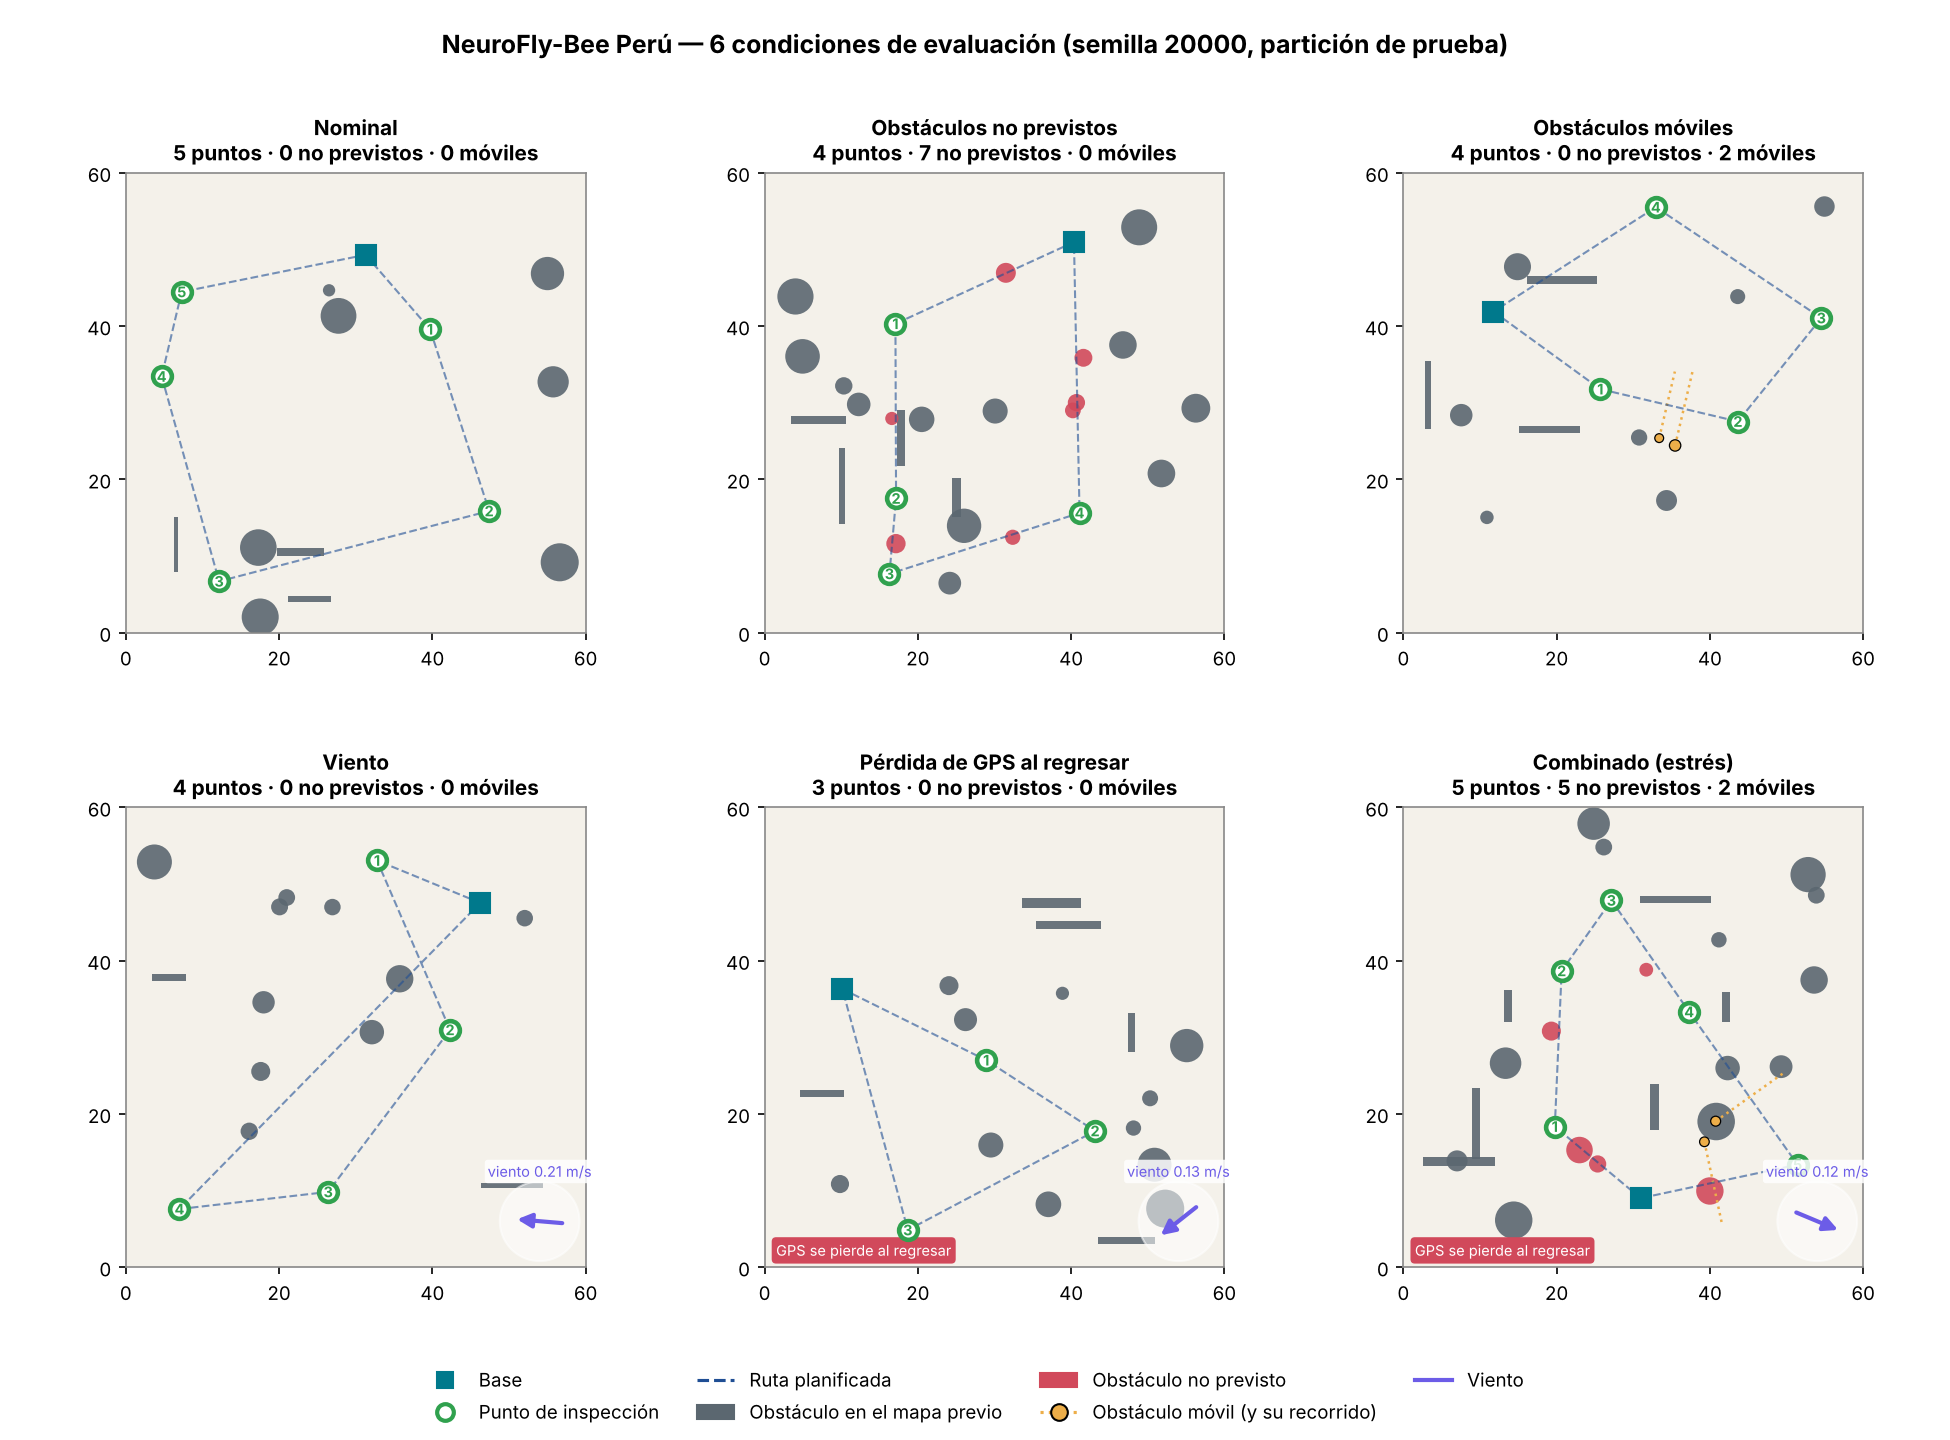
\includegraphics[width=0.85\textwidth]{v3_escenarios}
\caption{Las seis condiciones para una misma semilla de prueba. Gris: obstáculos del mapa
previo; rojo: no previstos; naranja: móviles con su recorrido; verde: puntos de inspección.}
\label{fig:escenarios}
\end{figure*}

\begin{figure*}[t]
\centering
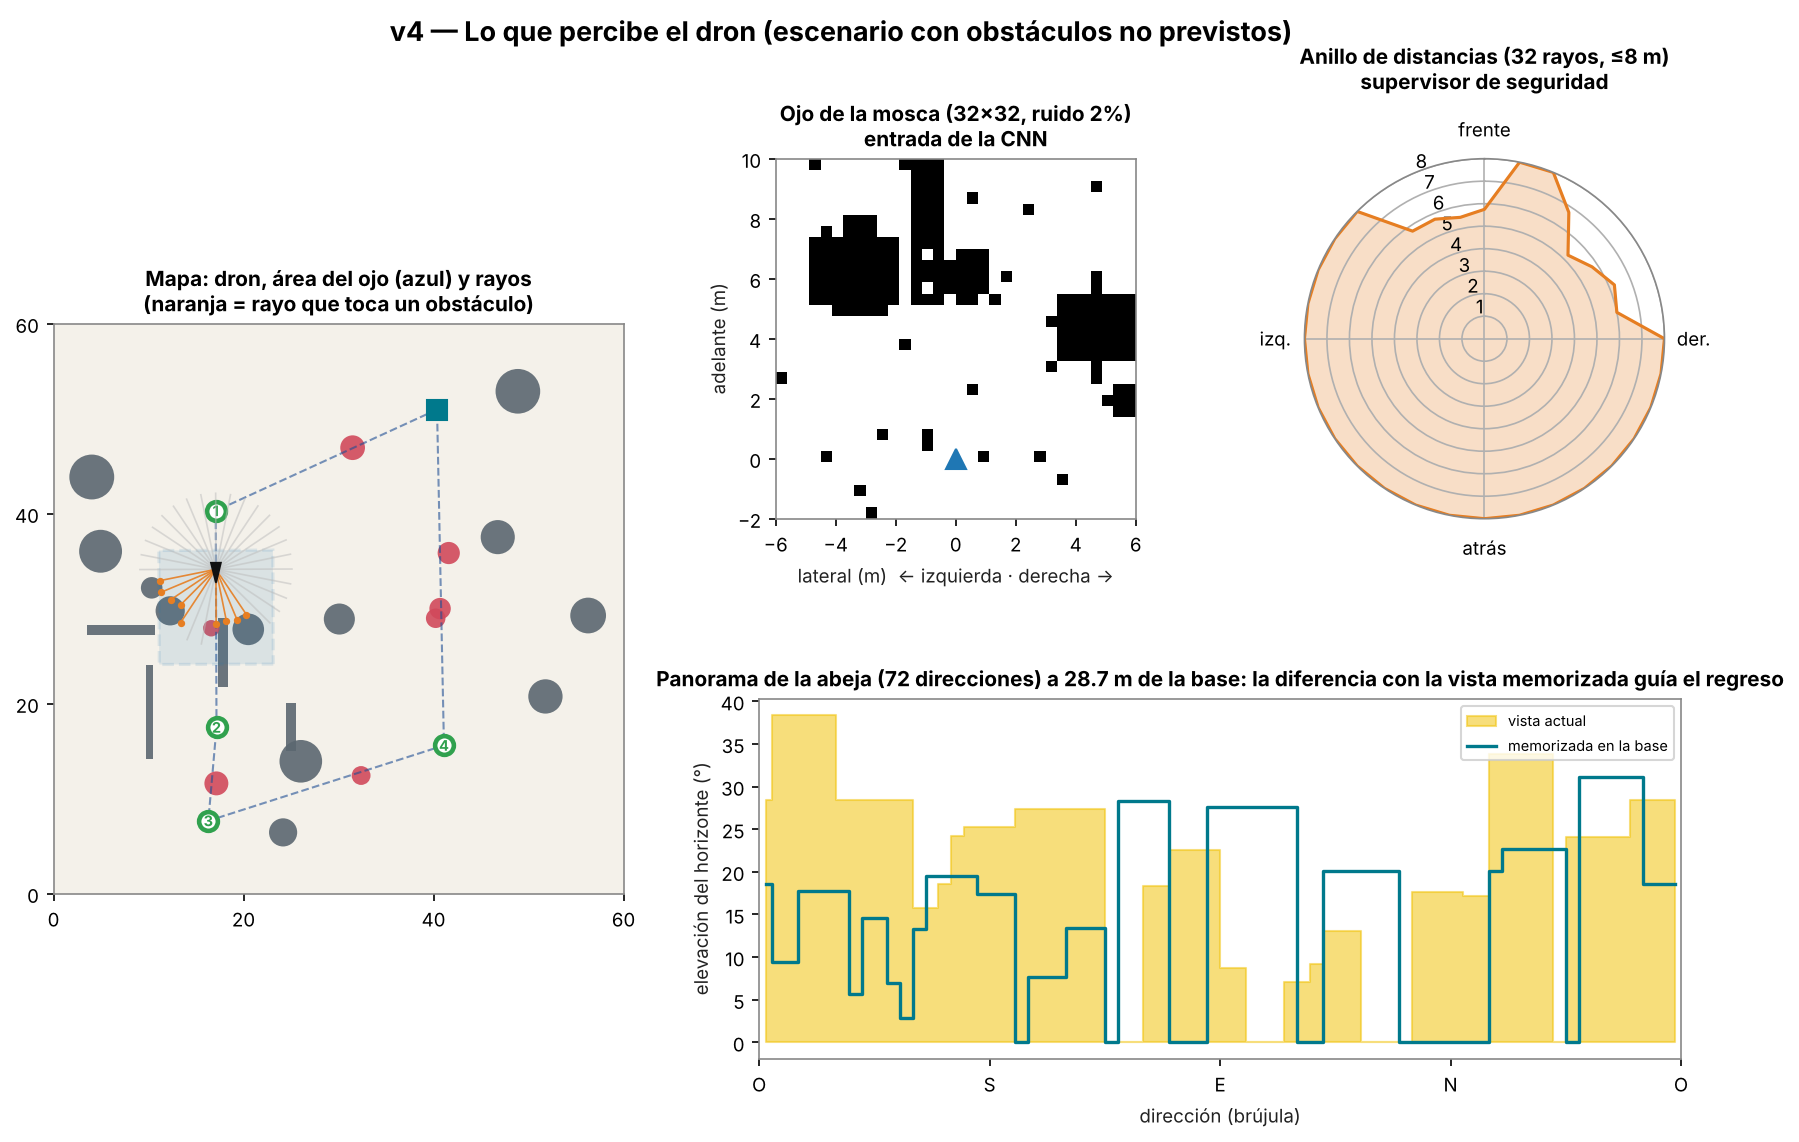
\includegraphics[width=0.9\textwidth]{v4_sensores}
\caption{Lo que percibe el dron: área del ojo y rayos sobre el mapa, ojo de la mosca (entrada
de la CNN), anillo de distancias (supervisor) y panorámica de la abeja.}
\label{fig:sensores}
\end{figure*}

\begin{figure*}[t]
\centering
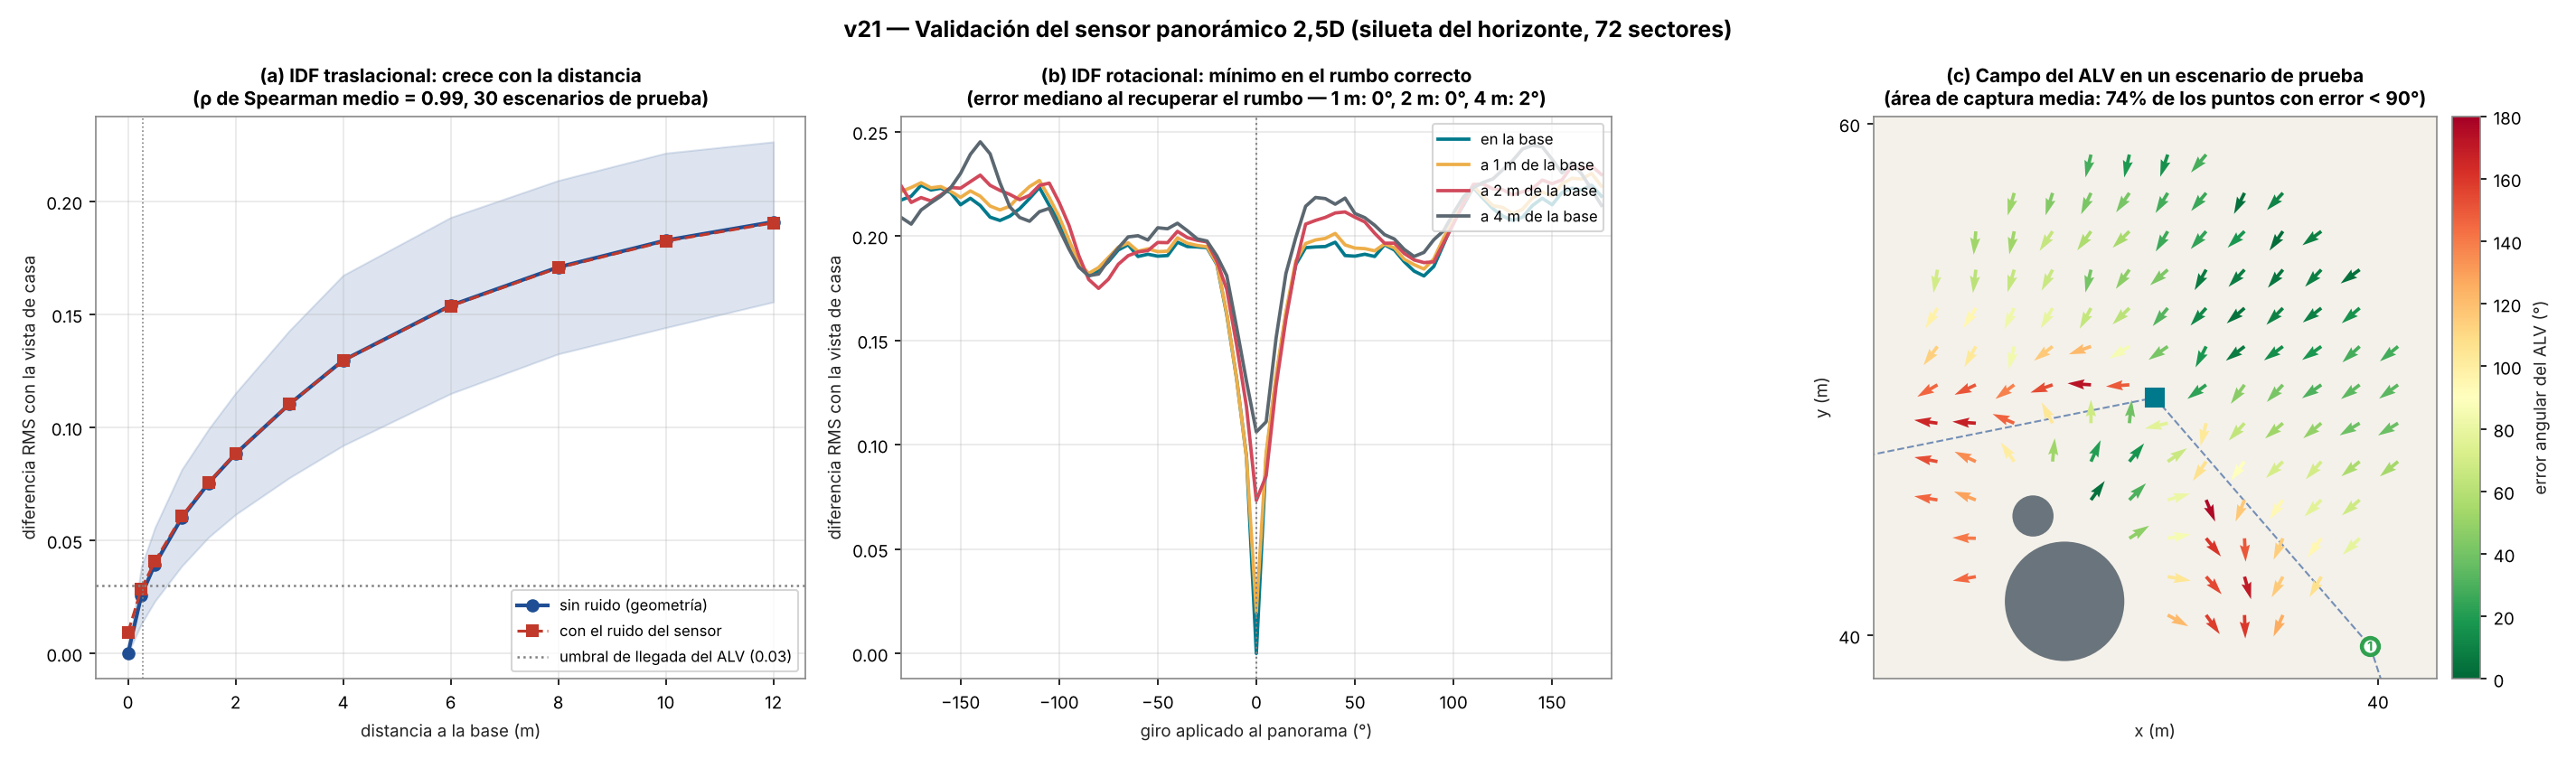
\includegraphics[width=\textwidth]{v21_validacion_sensor}
\caption{Validación del sensor panorámico 2.5D en escenarios de prueba: (a) IDF traslacional
(media $\pm$ d.e.) sin ruido y con el ruido del sensor; (b) IDF rotacional en la base y a 1,
2 y 4\,m; (c) campo del ALV coloreado por su error angular.}
\label{fig:sensor}
\end{figure*}

% Sección del artículo — dueño: P4.
\subsection{Líneas base}
Todas las líneas base usan la misma interfaz de controlador y las mismas observaciones que el
dron (nunca la información privilegiada del experto): \emph{directo} (vuela en línea recta
hacia el objetivo), \emph{campos de potencial}~\cite{khatib1986} (atracción al objetivo y
repulsión de los rayos), \emph{A*}~\cite{hart1968} con replanificación sobre el mapa previo
actualizado con los rayos, \emph{A* + ALV}, que al perder el GPS vuelve con el vector
promedio de hitos~\cite{lambrinos2000}, y \emph{A* + supervisor}. Sin GPS todas estiman su
posición integrando brújula y odometría (Fig.~\ref{fig:lineasbase}).

\begin{figure}[t]
\centering
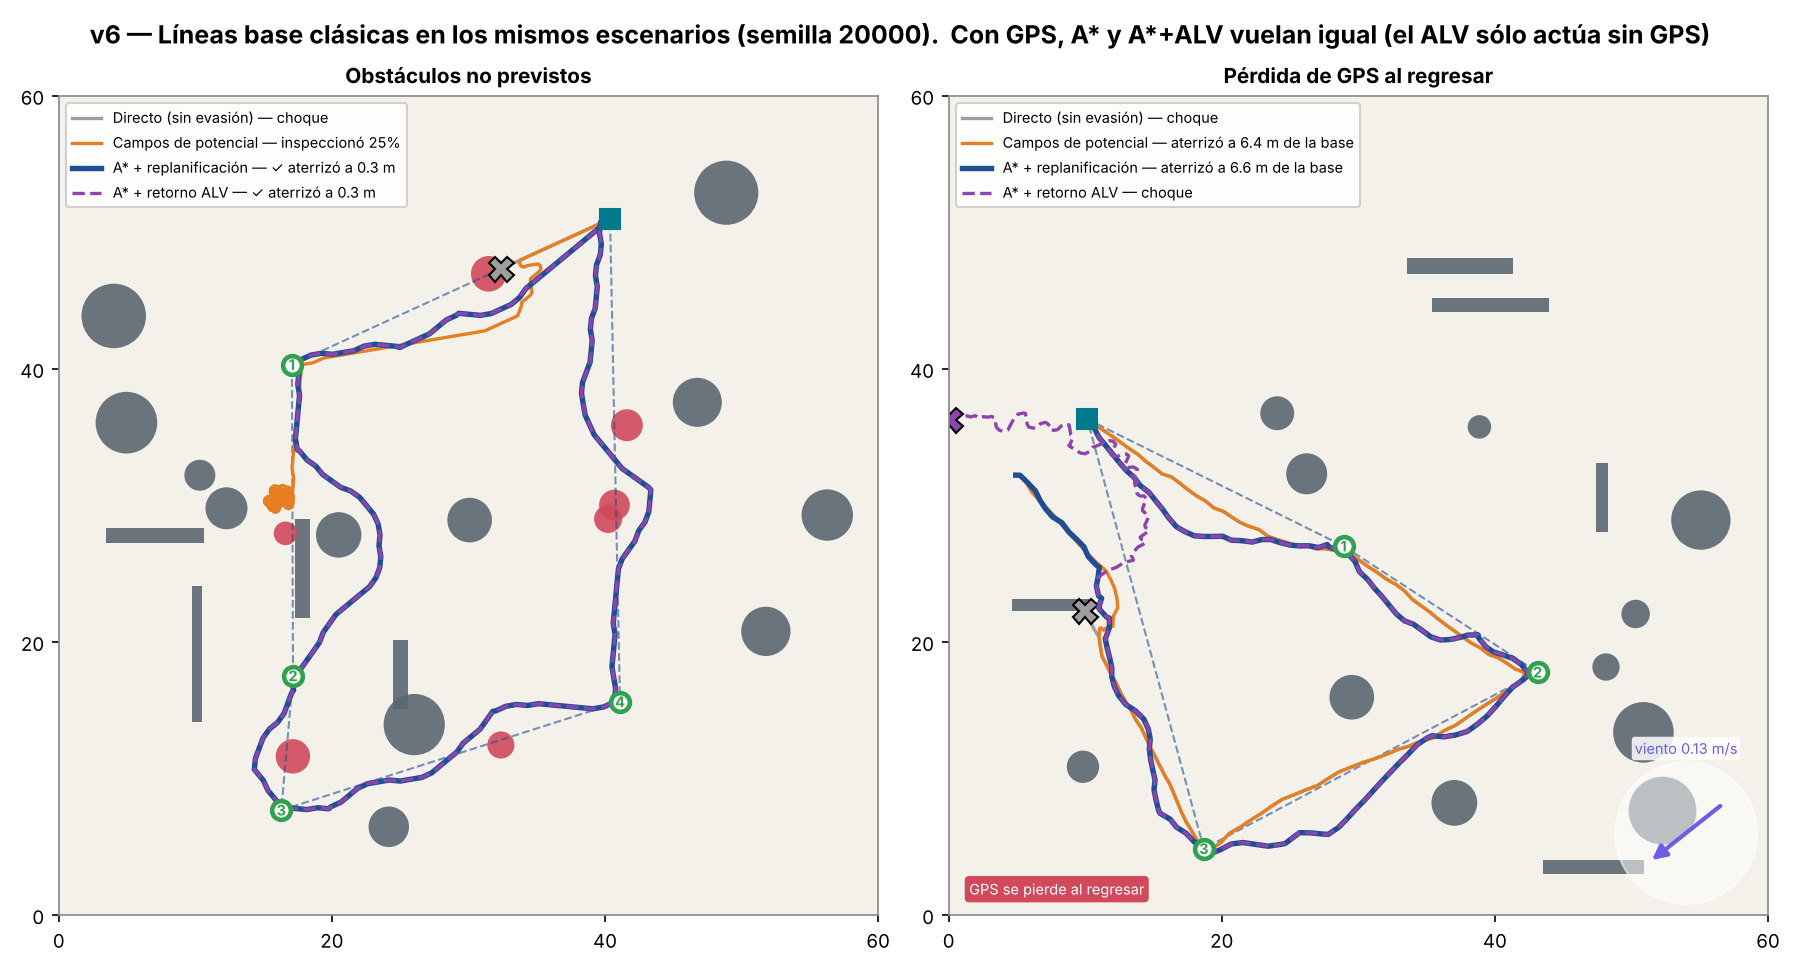
\includegraphics[width=\linewidth]{v6_lineas_base}
\caption{Líneas base en un mismo escenario. Sin GPS, la deriva hace que aterricen lejos de la
base o choquen.}
\label{fig:lineasbase}
\end{figure}

% Sección del artículo — dueño: P5. Sólo el dueño edita este archivo (v18).
\subsection{Arquitectura propuesta}
\textbf{Módulo mosca.} Cada cuadro del ojo $x_\tau\in\{0,1\}^{32\times32}$ pasa por un
codificador convolucional compartido $\phi$ (tres bloques conv$3\times3$--BN--ReLU--MaxPool
con 16, 32 y 64 filtros, y una capa lineal a 128 dimensiones). Una GRU~\cite{cho2014}
integra la secuencia de los últimos $T=4$ cuadros,
\begin{equation}
h_\tau = \mathrm{GRU}\big(\phi(x_\tau), h_{\tau-1}\big),\qquad \tau = t-T+1,\dots,t,
\end{equation}
y la decisión se toma con el último estado y el objetivo relativo codificado $g_t$:
$p_\theta(a\mid x_{t-T+1:t}, g_t) = \mathrm{softmax}\big(f([h_t; \psi(g_t)])\big)$.
Como comparación se usan un MLP (\nfbParamsMLP{} parámetros) y una CNN de un solo cuadro
(\nfbParamsCNN{}), y una variante con un codificador Transformer~\cite{vaswani2017}
(\nfbParamsTransformer{}) en lugar de la GRU; la propuesta CNN+GRU tiene \nfbParamsGRU{}
parámetros (Fig.~\ref{fig:redesmosca}).

\begin{figure*}[t]
\centering
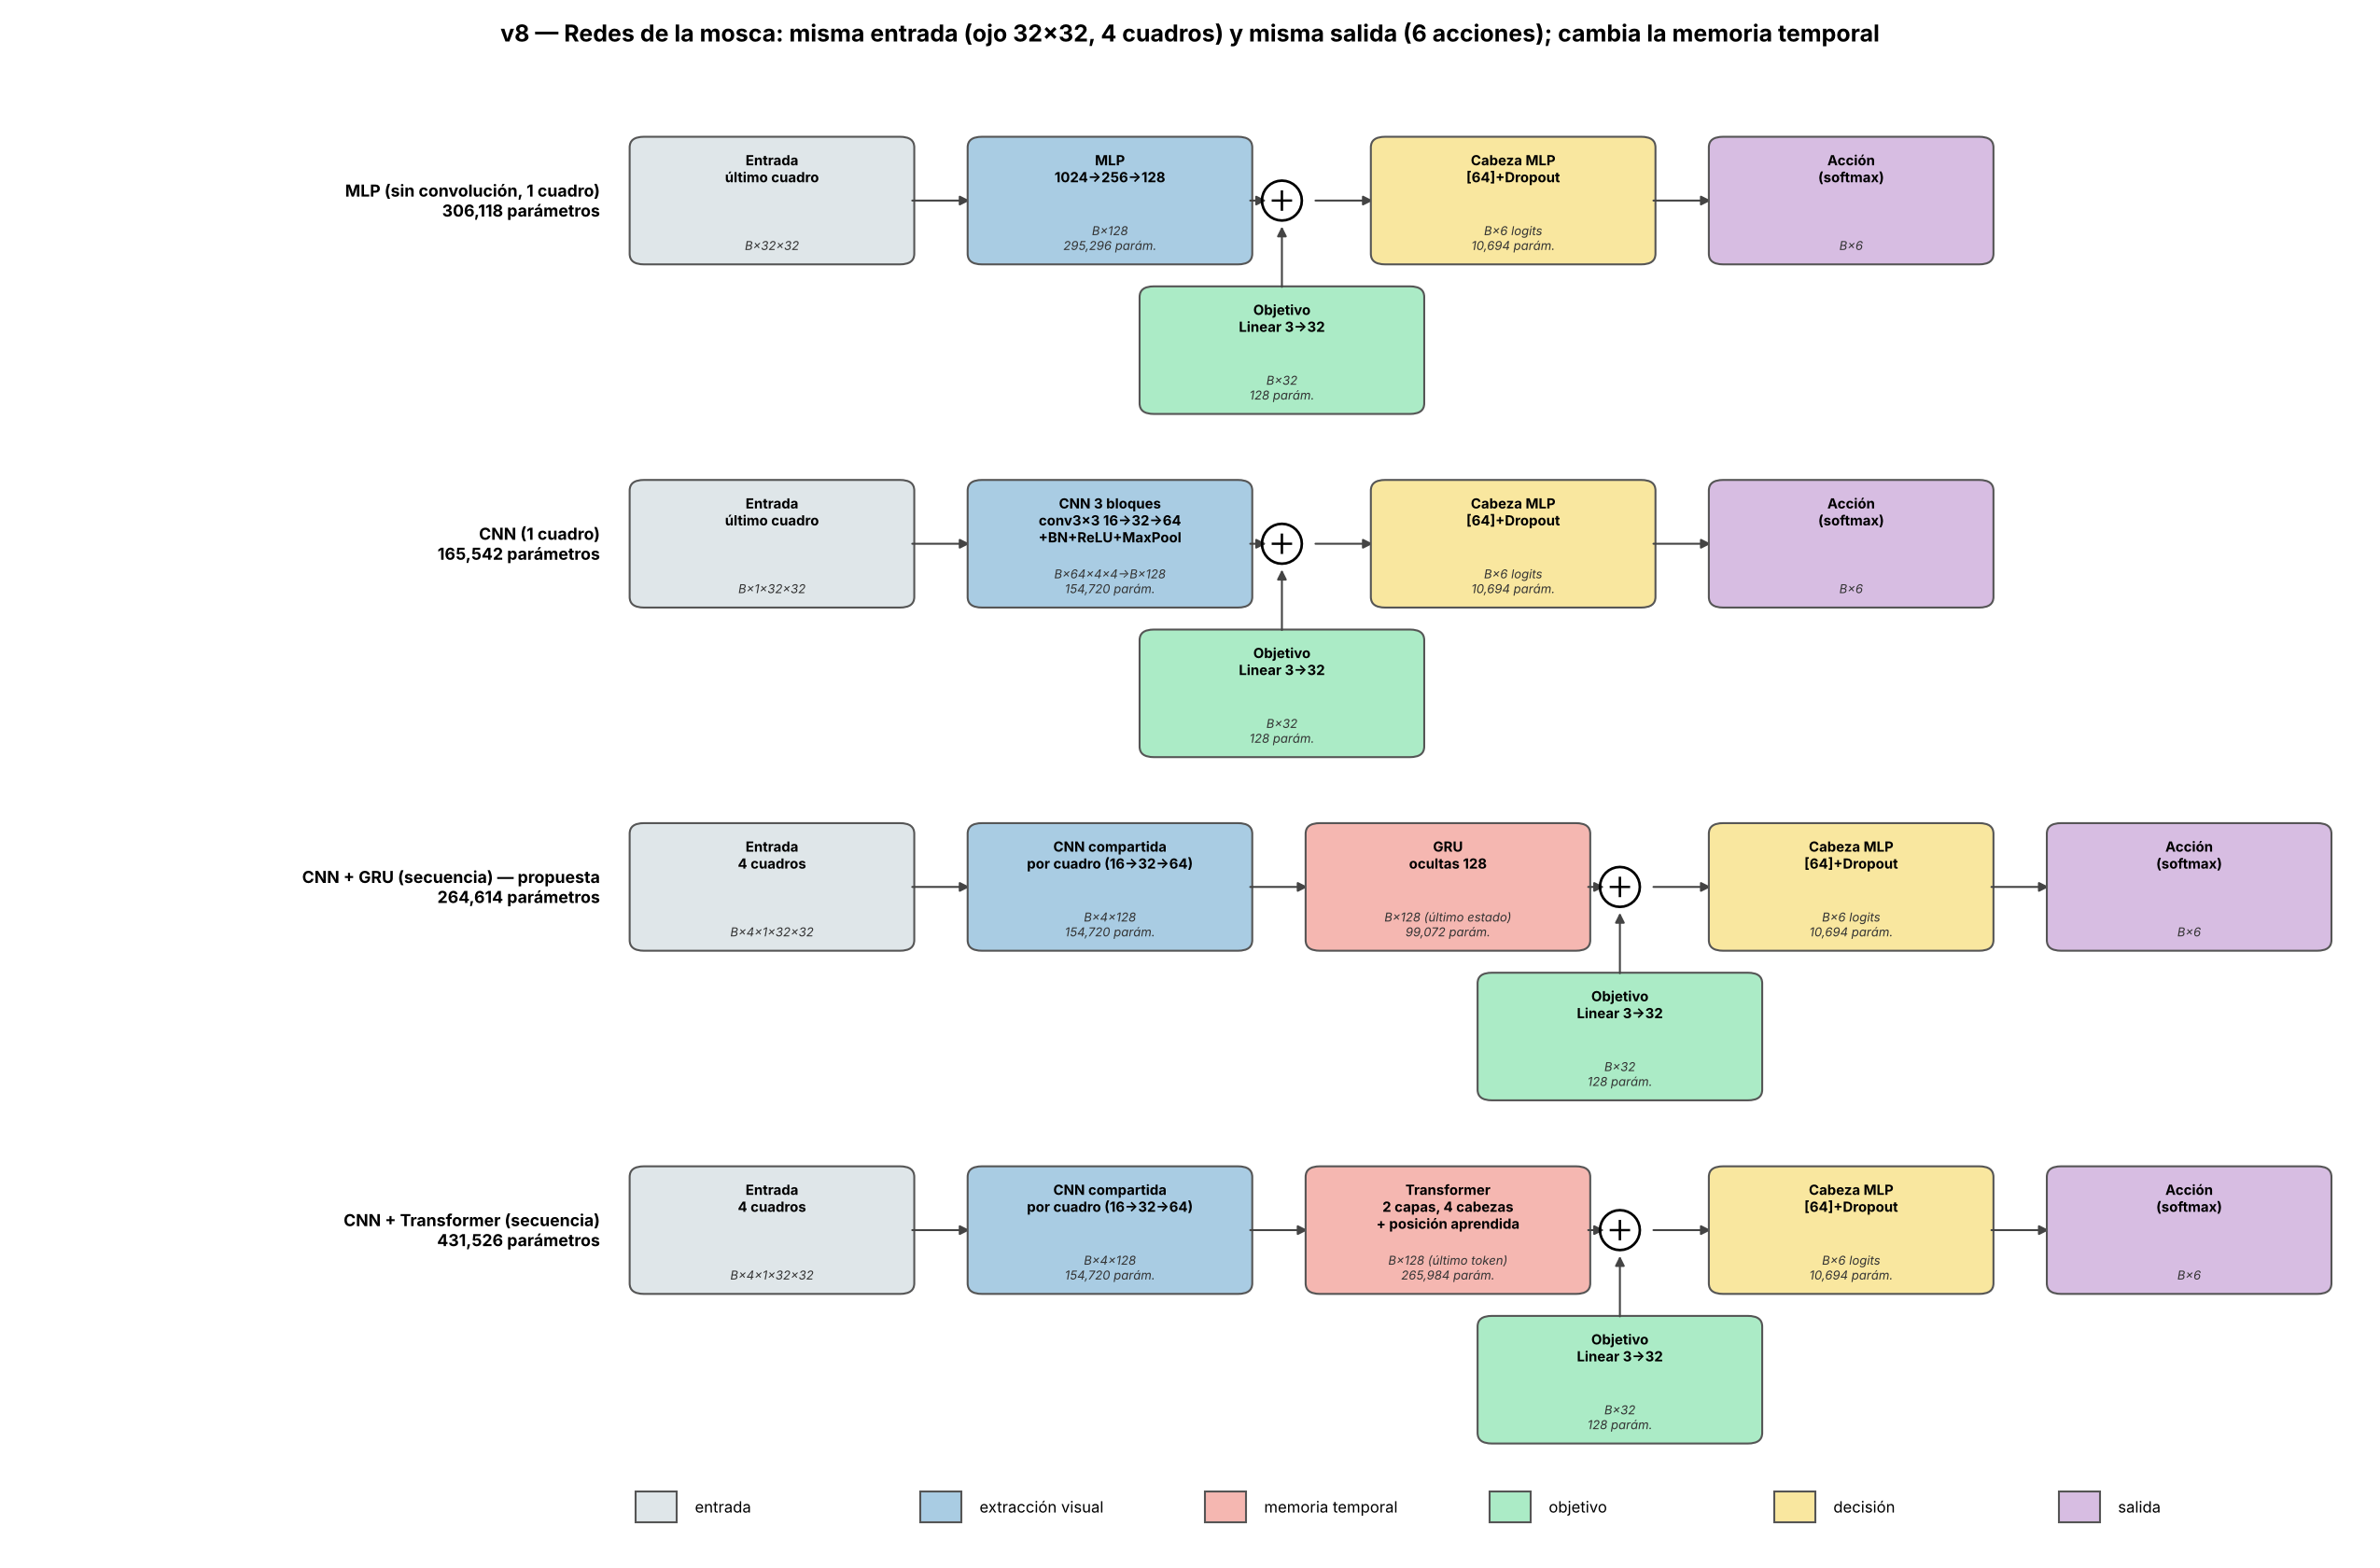
\includegraphics[width=0.95\textwidth]{v8_redes_mosca}
\caption{Redes del módulo mosca: misma entrada y salida; cambia la memoria temporal.}
\label{fig:redesmosca}
\end{figure*}

\textbf{Módulo abeja.} Inspirado en el modelo de instantáneas de las abejas~\cite{cartwright1983},
el dron memoriza al despegar la silueta panorámica de la base $s_0\in[0,1]^{72}$, alineada
con la brújula. Una red siamesa 1D $\rho$ con relleno circular codifica la vista actual $s_t$
y la memorizada; la cabeza recibe $[\rho(s_t);\rho(s_0);\rho(s_t)-\rho(s_0)]$ y predice
$(\cos\hat\theta,\sin\hat\theta,\log(1+\hat d))$, la dirección y la distancia a la base.
Se entrena minimizando
\begin{equation}
\begin{split}
\mathcal{L}_{\text{abeja}} ={}& \big(1-\cos(\hat\theta-\theta)\big)\\
&+ \lambda\,\mathrm{SmoothL1}\big(\log(1+\hat d),\log(1+d)\big),\quad \lambda=0.5.
\end{split}
\label{eq:abeja}
\end{equation}
La cabeza aplana el mapa de rasgos ($64\times18$) y lo pasa por un MLP con
\emph{dropout} de 0.1; concentra 148\,000 de los 172\,547 parámetros. Para la ablación se
definen tres variantes que cambian una sola decisión: sólo la vista actual, sin la resta
$\rho(s_t)-\rho(s_0)$, y una \emph{lectura vectorial} compacta en la que cada uno de los 18
sectores (centro $\varphi_k$) emite un voto $w_k$ y la dirección es
$\hat{\mathbf v}=\sum_k w_k(\cos\varphi_k,\sin\varphi_k)$, como el ALV pero con pesos
aprendidos (\nfbParamsAbejaCompacta{} parámetros en total).
La línea base es el vector promedio de hitos (ALV)~\cite{lambrinos2000}, que con las mismas
entradas obtiene un error angular mediano de \nfbAlvErrorMediano{} en validación (Fig.~\ref{fig:abeja}).

\begin{figure*}[t]
\centering
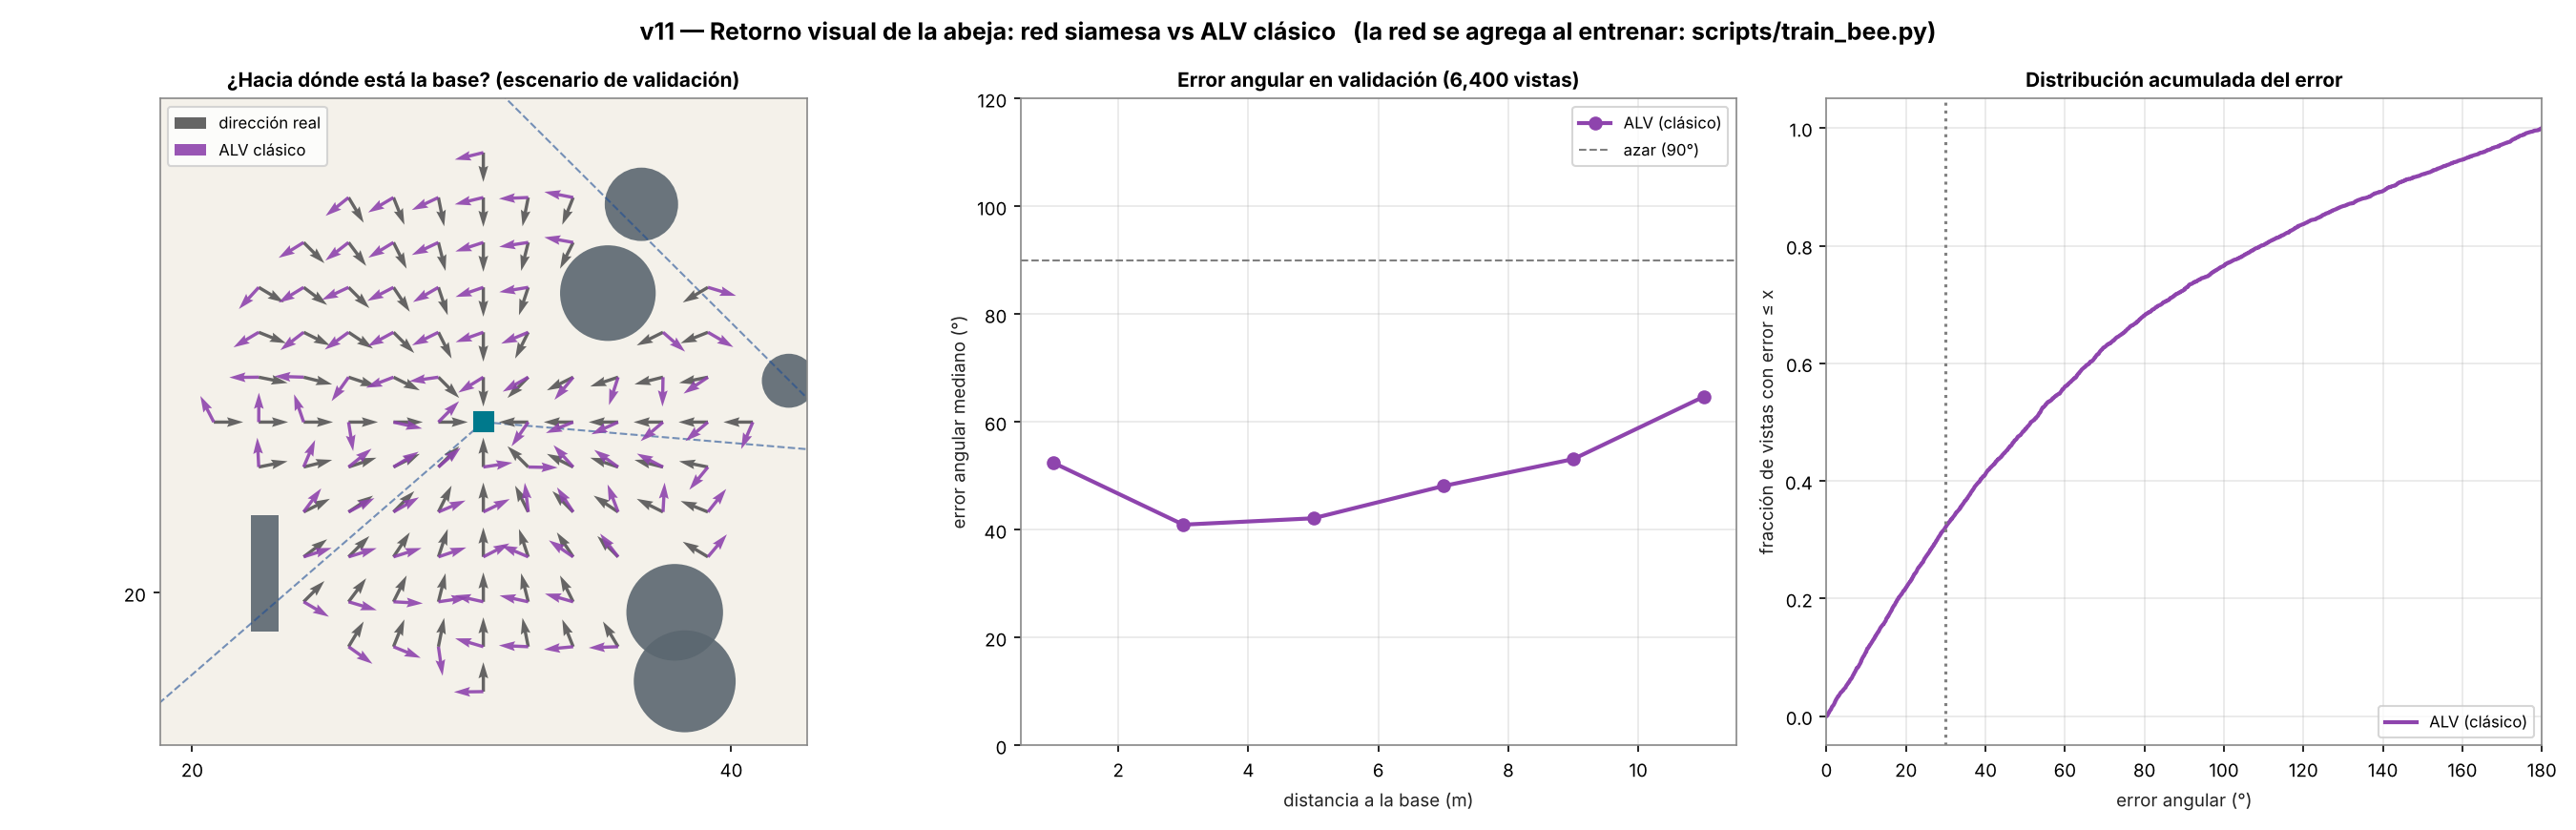
\includegraphics[width=0.95\textwidth]{v11_retorno_abeja}
\caption{Retorno visual: dirección real, ALV clásico y red de la abeja (validación).}
\label{fig:abeja}
\end{figure*}

\textbf{Integración y seguridad.} La abeja actúa como navegador de alto nivel (memoria
de la ruta, fase de la misión y, sin GPS, retorno visual), la mosca como control local y un
supervisor independiente de las redes veta, usando sólo el anillo de distancias, las
maniobras cuya posición prevista quede a menos de $r+0.6$\,m de un obstáculo detectado
(Fig.~\ref{fig:hibrido}). Con el controlador directo, el supervisor reduce los choques con
obstáculos fijos de \nfbChoquesDirectoFijos{} a \nfbChoquesDirectoSupFijos{}, pero no evita
los choques con obstáculos móviles, que llegan desde fuera del alcance de los rayos.

\begin{figure*}[t]
\centering
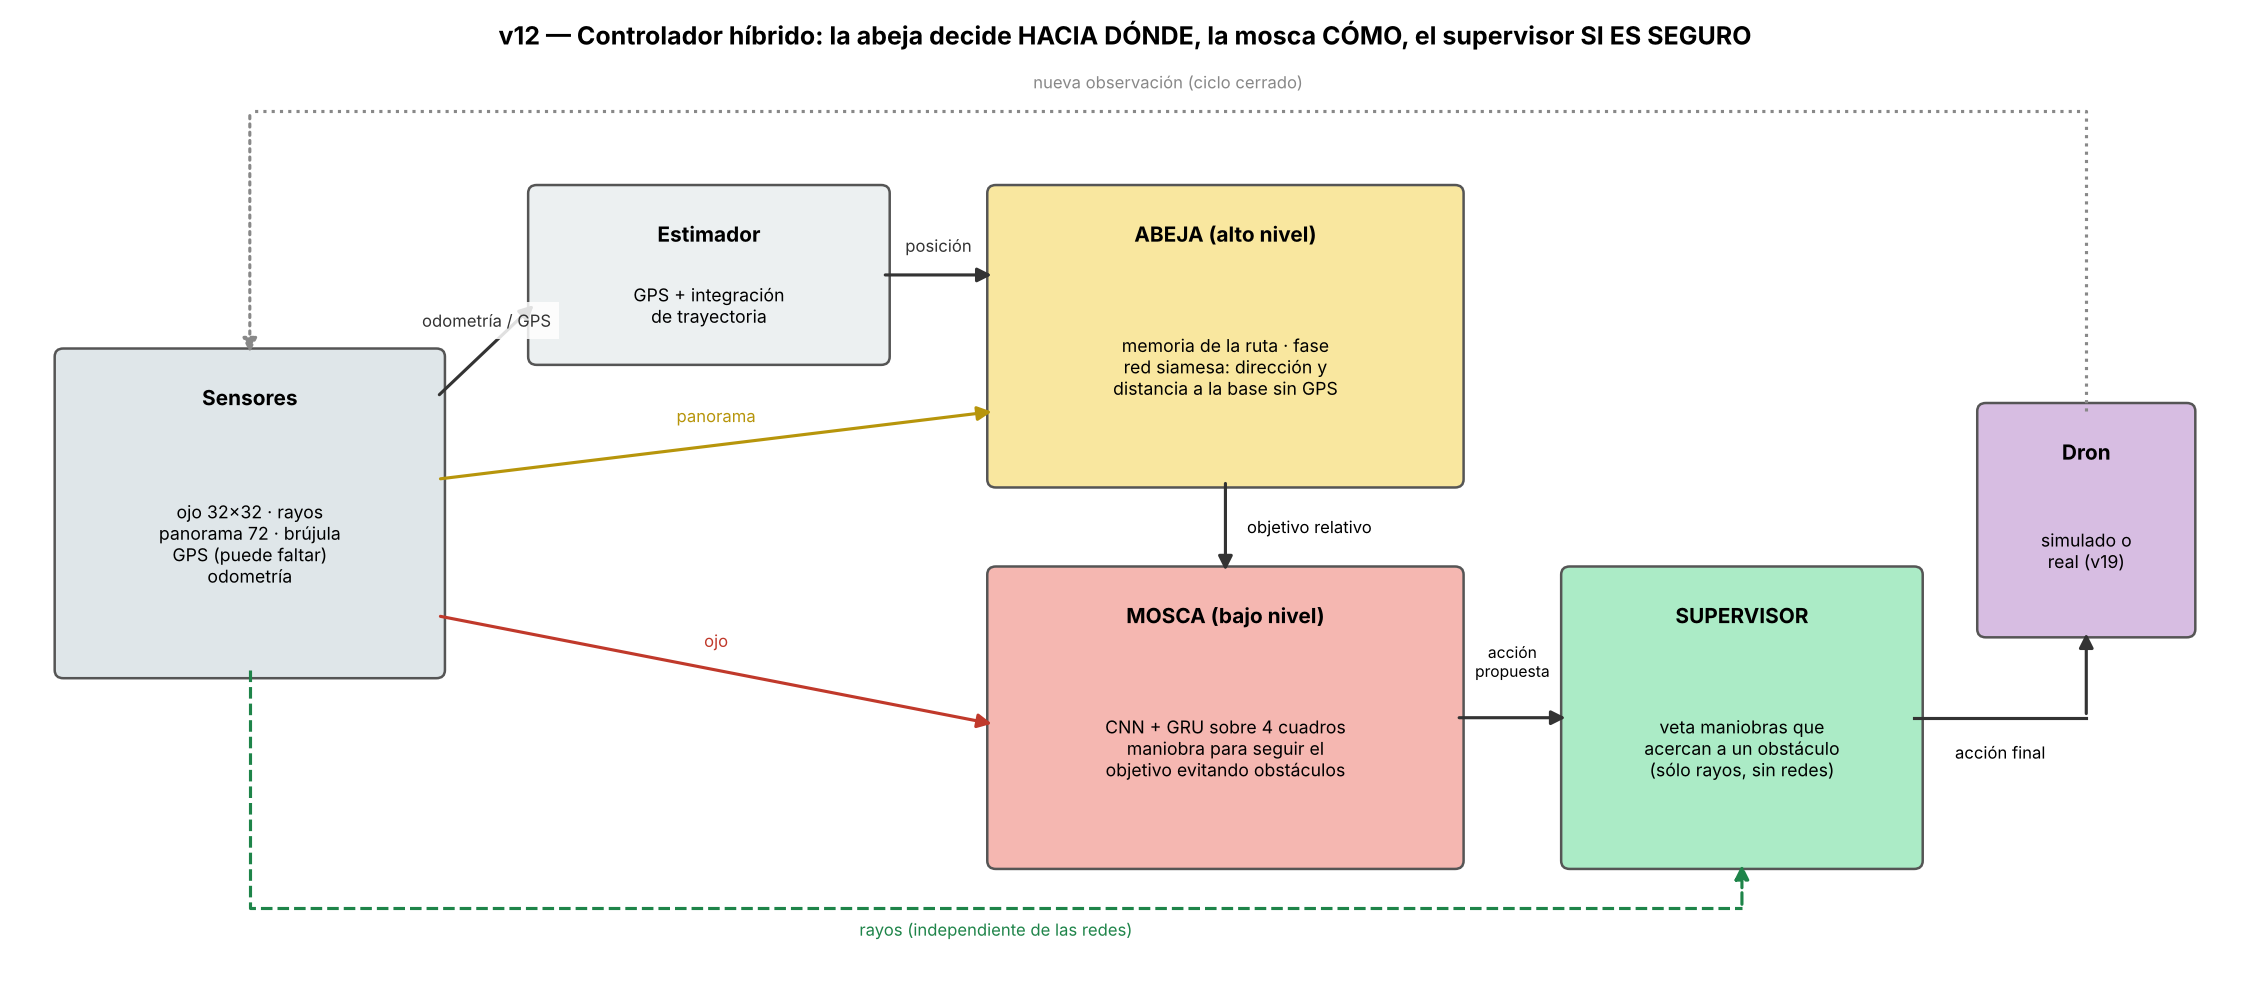
\includegraphics[width=0.9\textwidth]{v12_arquitectura_hibrida}
\caption{Controlador híbrido: abeja (hacia dónde), mosca (cómo) y supervisor (si es seguro).}
\label{fig:hibrido}
\end{figure*}

% Sección del artículo — dueño: P5. Sólo el dueño edita este archivo (v18).
\subsection{Formulación y funciones de pérdida}
La mosca minimiza la entropía cruzada ponderada por clase sobre las acciones del experto,
\begin{equation}
\mathcal{L}_{\text{mosca}}(\theta) = -\frac{1}{N}\sum_{i=1}^{N}\sum_{c=1}^{C}
w_c\, y_{i,c}\log p_\theta(c \mid x_{i,t-T+1:t}, g_i)
\label{eq:mosca}
\end{equation}
y la abeja la pérdida~\eqref{eq:abeja}.

\subsection{Entrenamiento y métricas}
Las redes de la mosca se entrenan por clonación de comportamiento sobre las etiquetas del
experto, minimizando la entropía cruzada ponderada~\eqref{eq:mosca} con $w_c\propto f_c^{-1/2}$
(recortado a 10), pues las acciones están desbalanceadas (40\,\% \emph{avanzar} y
0.1\,\% \emph{mantener posición}). Se usa AdamW~\cite{loshchilov2019} (tasa $10^{-3}$, decaimiento de pesos
$10^{-4}$, programación coseno), lotes de 256, hasta 15 épocas con parada temprana
(paciencia 4) y se conserva el modelo con mejor F1 macro en validación; el conjunto de
prueba no interviene en ninguna decisión. Los gradientes se recortan a norma 1. Cada
configuración se entrena con 3 semillas. La abeja usa el mismo optimizador con lotes de 512,
hasta 30 épocas con paciencia 6 sobre el error angular mediano de validación y un aumento que
rota la vista actual $\pm1$ sector (error de brújula de $\pm5$\textdegree).

Para mitigar el desplazamiento de distribución de la clonación de comportamiento se
aplica DAgger~\cite{ross2011} (Fig.~\ref{fig:dagger}): en la iteración $k$ la política
ejecutada es $\pi_k=\beta_k\pi^*+(1-\beta_k)\hat\pi_{k-1}$ con
$\beta=(0.5,\,0.25,\,0)$, el experto $\pi^*$ etiqueta los estados visitados, el conjunto
se agrega ($\mathcal D\leftarrow\mathcal D\cup\mathcal D_k$, 120 escenarios nuevos de
entrenamiento por iteración) y la red se reentrena 5 épocas desde los pesos anteriores.

\begin{figure}[t]
\centering
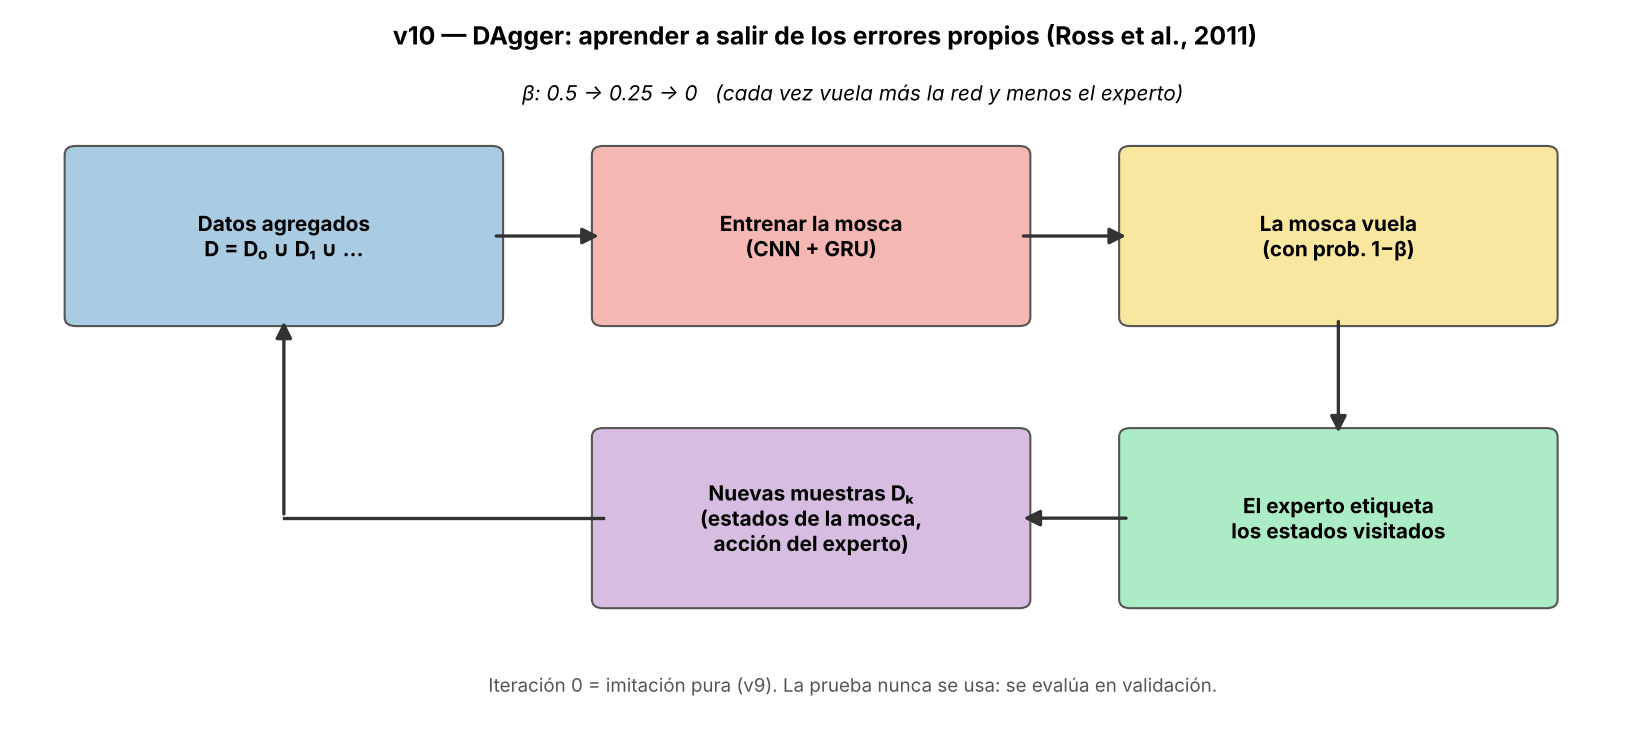
\includegraphics[width=\linewidth]{v10_dagger_esquema}
\caption{Ciclo de DAgger aplicado al módulo mosca.}
\label{fig:dagger}
\end{figure}
\textbf{Métricas.} Fuera de línea se reporta el F1 macro de validación, adecuado para
clases desbalanceadas (la exactitud premiaría avanzar siempre), y el AUROC macro uno contra
el resto~\cite{fawcett2006}, que mide si la red ordena bien las acciones con independencia del
umbral. La abeja se mide en grados (error angular mediano y fracción de vistas con error
$\le30$\textdegree), en la partición de prueba. En lazo cerrado, sobre las
semillas de prueba, se reportan la tasa de éxito de misión con su intervalo de Wilson al
95\,\%, la tasa de choques, el error de aterrizaje respecto de la base y la latencia por
decisión; para los controladores neuronales, la media $\pm$ desviación estándar entre las tres
semillas de entrenamiento.

\textbf{Significancia.} Como todos los controladores vuelan los mismos escenarios, las
comparaciones son pareadas: para cada escenario se toma el éxito de A y de B (media entre
semillas en los neuronales) y se analiza la diferencia $d_i$. Se reporta la media de $d_i$
con un IC 95\,\% bootstrap que remuestrea escenarios~\cite{efron1993}, el valor $p$ de una
prueba de permutación por cambio de signo (exacta, equivalente a McNemar, cuando $d_i\in\{-1,0,1\}$),
corregido por Holm~\cite{holm1979} sobre todas las comparaciones, y la $h$ de
Cohen~\cite{cohen1988} como tamaño de efecto.

% Sección del artículo — dueño: P4.
\section{Resultados}
\subsection{Comparación con las líneas base}
La Tabla~\ref{tab:principal} y la Fig.~\ref{fig:benchmark} resumen
\nfbEpisodiosPorCondicion{} escenarios de prueba por condición. Entre las líneas base, A* con
replanificación resuelve casi todas las misiones con obstáculos fijos
(\nfbExitoAstarNominal{} nominal, \nfbExitoAstarDesconocidos{} con obstáculos no previstos),
pero sólo el \nfbExitoAstarMoviles{} con obstáculos móviles, porque planifica sobre una
fotografía del mapa que queda obsoleta. Sin GPS ninguna supera el
\nfbMejorClasicoSinGPS{}: A* aterriza donde \emph{cree} que está la base, y la deriva de la
odometría lo deja lejos; el retorno ALV corrige parte de ella (\nfbExitoAstarAlvSinGPS{} sin
GPS y \nfbExitoAstarAlvCombinado{} en la condición combinada, frente a \nfbExitoAstarSinGPS{} y
\nfbExitoAstarCombinado{} de A*). Los campos de potencial chocan poco
(\nfbChoquesCampos{}) pero se atascan en mínimos locales.

El híbrido NeuroFly-Bee obtiene \nfbExitoHibridoTotal{} de éxito total
(\nfbExitoHibridoMoviles{} con obstáculos móviles y \nfbExitoHibridoSinGPS{} sin GPS), frente
a \nfbExitoMoscaTotal{} de la mosca sola y \nfbExitoAbejaTotal{} de A* con la red de la abeja.
% P4: comentar aquí, con los números de v19, si el híbrido supera a A*+ALV y dónde no.

\begin{table*}[t]
\centering
\caption{Éxito de misión en la partición de prueba (media $\pm$ d.e. entre semillas de entrenamiento para los controladores neuronales) y tasa total de choques.}
\label{tab:principal}
\begin{tabular}{lcccccccc}
\toprule
Controlador & Nominal & No previstos & Móviles & Viento & Sin GPS & Combinado & Total & Choques \\
\midrule
Directo & 7\% & 0\% & 0\% & 13\% & 0\% & 0\% & 3\% & 95\% \\
Campos de potencial & 77\% & 57\% & 77\% & 80\% & 0\% & 0\% & 48\% & 3\% \\
A* (clásico) & 100\% & 97\% & 40\% & 93\% & 3\% & 0\% & 56\% & 16\% \\
A* + ALV (clásico) & 100\% & 97\% & 40\% & 93\% & 17\% & 23\% & \textbf{62\%} & 16\% \\
A* + supervisor & 100\% & 100\% & 53\% & 93\% & 3\% & 0\% & 58\% & 12\% \\
\bottomrule
\end{tabular}
\end{table*}


\begin{figure*}[t]
\centering
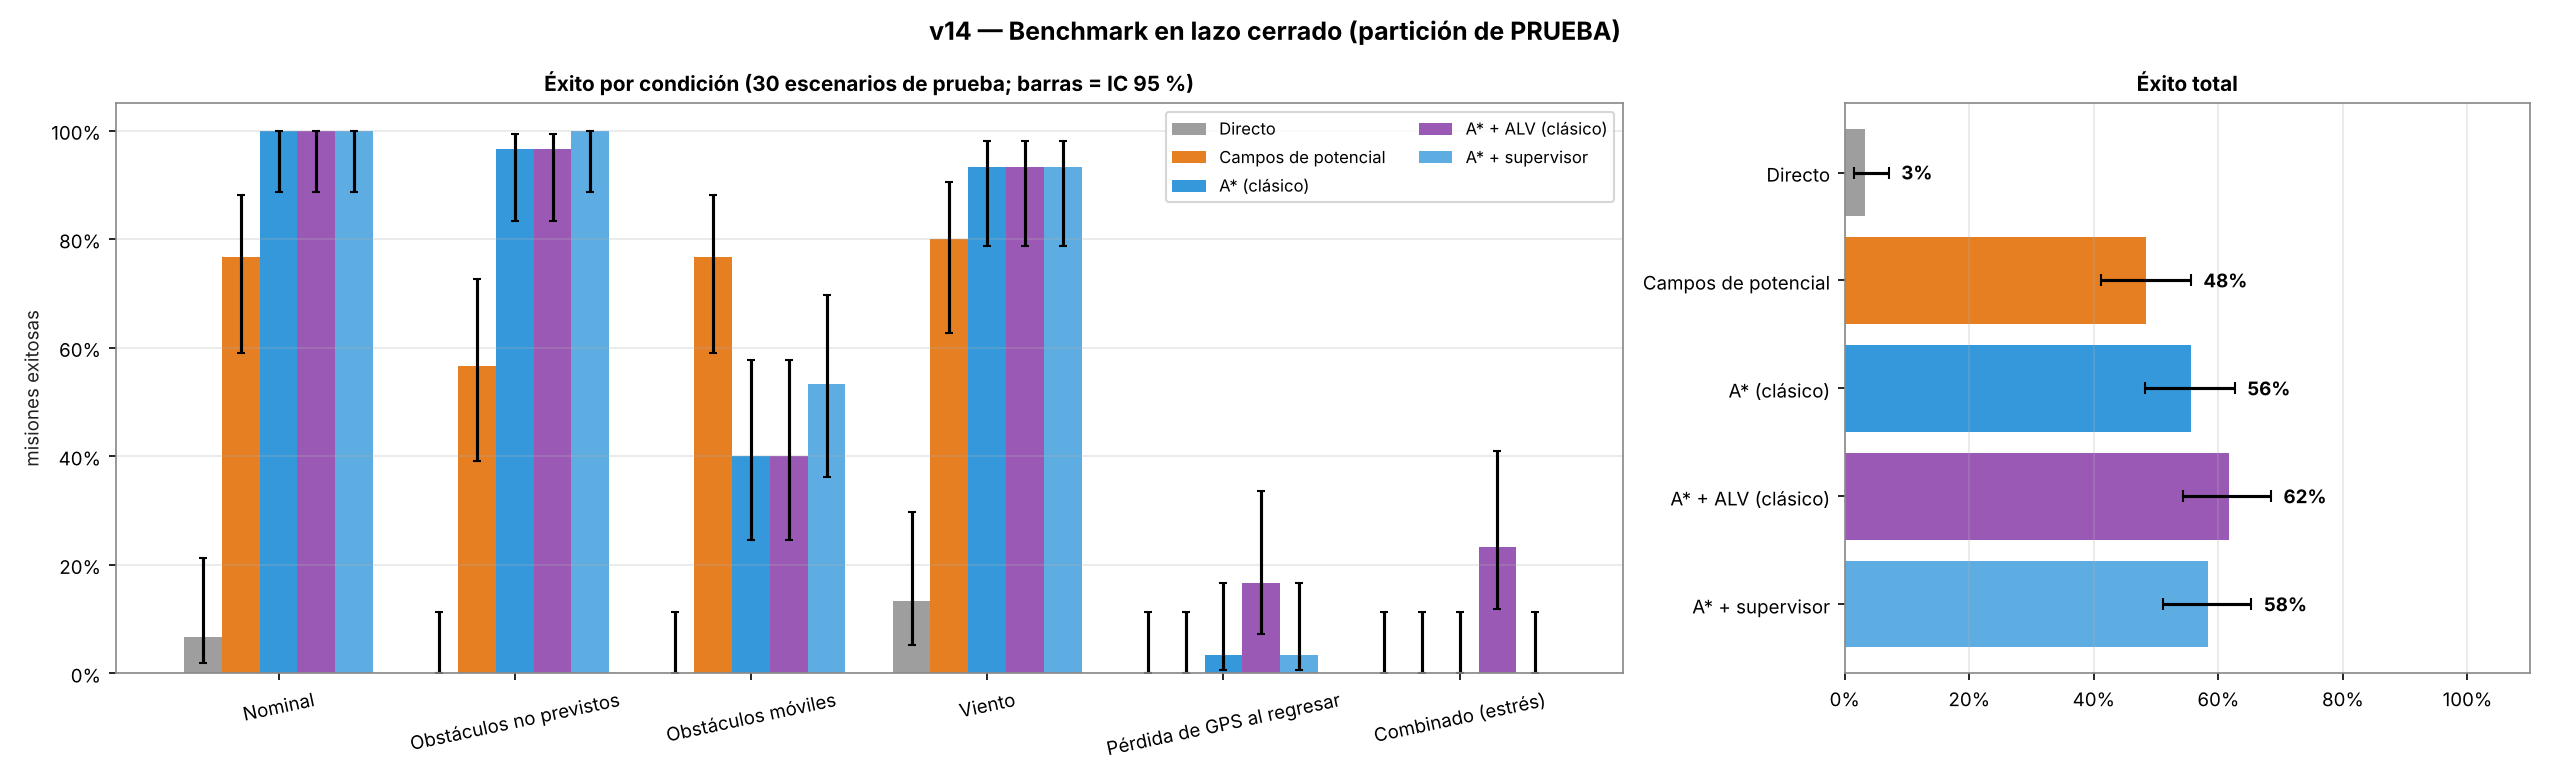
\includegraphics[width=0.9\textwidth]{v14_benchmark}
\caption{Éxito de misión por condición en la partición de prueba (barras de error: IC de
Wilson al 95\,\%).}
\label{fig:benchmark}
\end{figure*}

\subsection{Estudio de ablación}
Cuatro ablaciones aíslan cada decisión de diseño con las mismas semillas de prueba:
(i) arquitectura de la mosca con imitación pura (MLP, CNN, CNN+GRU, CNN+Transformer),
(ii) imitación frente a imitación + DAgger, (iii) retorno sin GPS (ninguno, ALV clásico y red
de la abeja) y (iv) aporte de cada módulo (mosca sola, abeja + mosca, abeja + mosca +
supervisor). En validación, el F1 macro de la mosca es \nfbFUnoMLP{} (MLP), \nfbFUnoCNN{}
(CNN), \nfbFUnoGRU{} (CNN+GRU) y \nfbFUnoTransformer{} (CNN+Transformer), con un AUROC macro
de \nfbAurocGRU{} para CNN+GRU; DAgger lleva el
éxito en lazo cerrado de \nfbDaggerExitoInicial{} a \nfbDaggerExitoFinal{}. La red de la abeja
obtiene en validación un error angular mediano de \nfbAbejaErrorMediano{} frente a
\nfbAlvErrorMediano{} del ALV. Las tablas de ablación del benchmark se regeneran con los pesos
de cada variante.

% Se incluyen las que existan (run_benchmark.py las regenera con los pesos).
\IfFileExists{tablas/v14_ablacion_1.tex}{\input{tablas/v14_ablacion_1}}{}
\IfFileExists{tablas/v14_ablacion_2.tex}{\input{tablas/v14_ablacion_2}}{}
\IfFileExists{tablas/v14_ablacion_3.tex}{\begin{table*}[t]
\centering
\caption{Retorno sin GPS}
\label{tab:ablacion3}
\begin{tabular}{lcccc}
\toprule
Controlador & Sin GPS & Combinado & Total & Choques \\
\midrule
A* sin retorno visual & 3\% & 0\% & 2\% & 17\% \\
A* + ALV clásico & 17\% & 23\% & \textbf{20\%} & 17\% \\
\bottomrule
\end{tabular}
\end{table*}
}{}
\IfFileExists{tablas/v14_ablacion_4.tex}{\input{tablas/v14_ablacion_4}}{}

\subsection{Ablación de la abeja en la partición de prueba}
La Tabla~\ref{tab:ablacion_abeja} y la Fig.~\ref{fig:ablacion_abeja} responden dos preguntas
sobre el diseño siamés, con las mismas semillas, datos e hiperparámetros y sobre
\nfbMuestrasAbejaTest{} vistas de prueba. \emph{¿Hace falta la vista de casa?} Sin ella, la
red obtiene \nfbAblAbejaVistaUnica{} de error mediano, frente a \nfbAblAbejaCompleta{} de la
siamesa; como cada mundo de prueba es distinto, una sola vista sólo puede indicar la base a
través de regularidades del generador de escenarios.
\emph{¿Hace falta la resta explícita?} Sin ella, \nfbAblAbejaSinResta{}.
\emph{¿Hacen falta 172\,547 parámetros?} La lectura vectorial, con
\nfbParamsAbejaCompacta{} parámetros (\nfbAbejaReduccionParams{} veces menos), obtiene
\nfbAblAbejaCompacta{}. El ALV clásico sobre las mismas vistas tiene \nfbAblAbejaAlv{}.
% P4: interpretar aquí con los números de Colab (si la compacta iguala a la plana, el
% argumento de tamaño frente a Bee-Nav queda resuelto).

\begin{table}[t]
\caption{Ablación de la red de la abeja en la partición de prueba (6\,400 vistas; media $\pm$ d.e. entre semillas)}
\label{tab:ablacion_abeja}
\centering
\resizebox{\linewidth}{!}{%
\begin{tabular}{lrrr}
\toprule
Variante & Parámetros & Error mediano (\textdegree) & Error $\le$30\textdegree{} \\
\midrule
ALV clásico & -- & 55.4 & 30\,\% \\
\bottomrule
\end{tabular}}
\end{table}


\begin{figure*}[t]
\centering
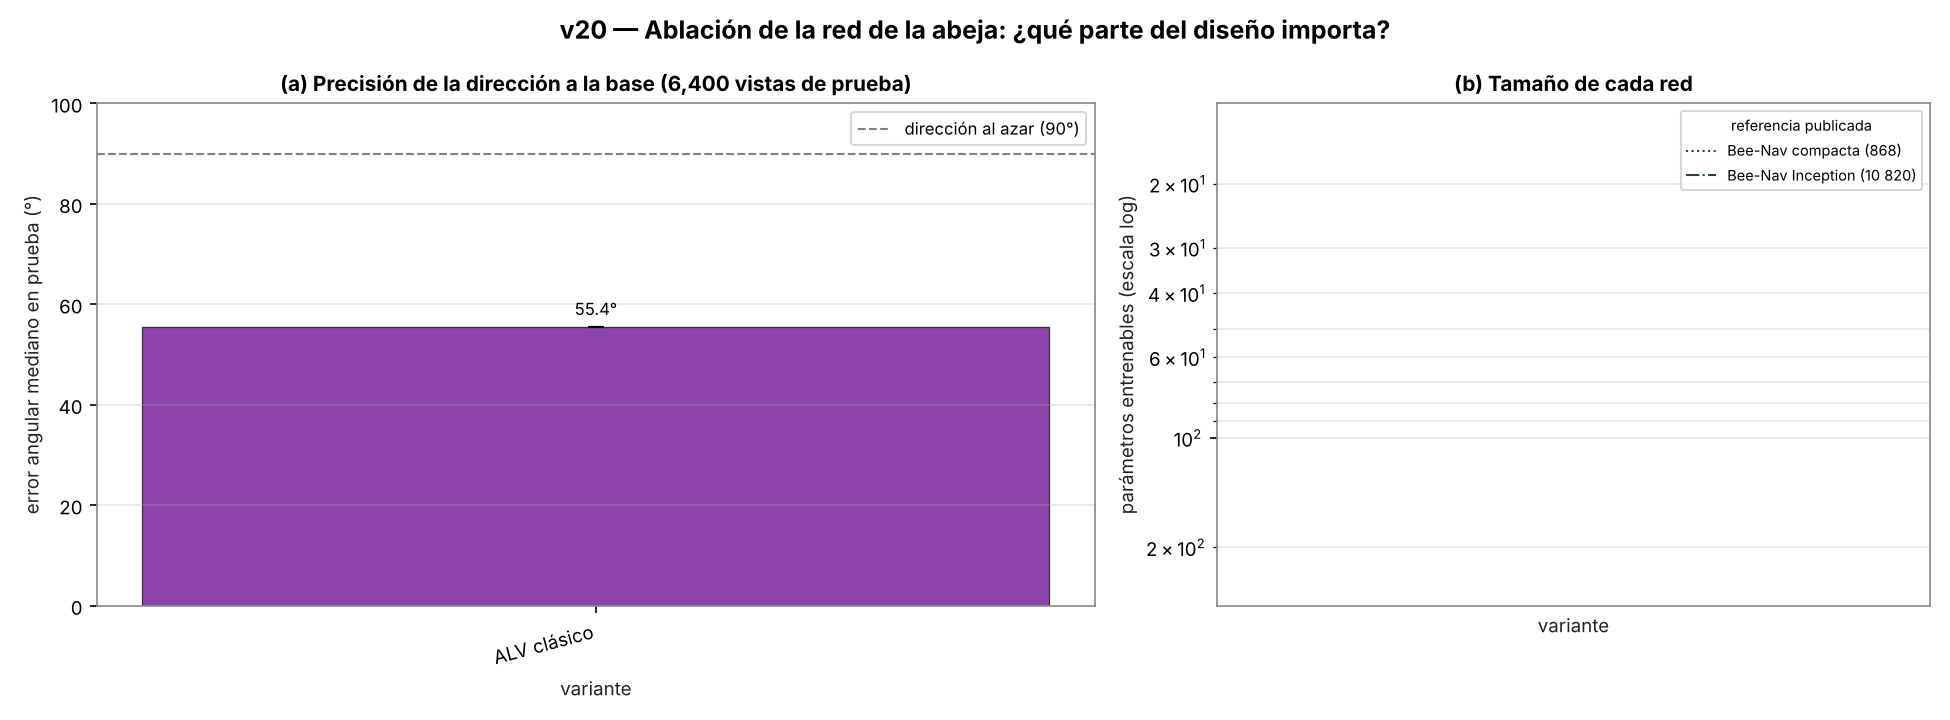
\includegraphics[width=0.95\textwidth]{v20_ablacion_abeja}
\caption{Ablación de la abeja en prueba: (a) error angular mediano (media $\pm$ d.e. entre
semillas; línea punteada: dirección al azar); (b) parámetros en escala logarítmica, con el
tamaño de las redes publicadas de Bee-Nav~\cite{ou2026} como referencia.}
\label{fig:ablacion_abeja}
\end{figure*}

\subsection{Significancia estadística}
La Tabla~\ref{tab:significancia} reúne las comparaciones pareadas;
\nfbSigSignificativas{} de \nfbSigComparaciones{} son significativas tras la corrección de
Holm. Entre las líneas base, el retorno ALV mejora a A* en \nfbSigAlvAstarTotalDif{} de
éxito total (\nfbSigAlvAstarTotalP{}). El híbrido frente a A*+ALV difiere en
\nfbSigHibridoAlvTotalDif{} en total (\nfbSigHibridoAlvTotalP{}) y en
\nfbSigHibridoAlvSinGPSDif{} sin GPS (\nfbSigHibridoAlvSinGPSP{}). Con 30 escenarios por
condición y una corrección conservadora, diferencias de unos 10 puntos pueden no alcanzar
significancia; por eso se reportan siempre el intervalo y el tamaño de efecto.

\begin{table*}[t]
\caption{Comparaciones pareadas sobre los mismos escenarios de prueba: diferencia de éxito $\Delta$ con IC 95\,\% bootstrap, valor $p$ de la permutación pareada corregido por Holm y $h$ de Cohen. En negrita, $p_{\text{Holm}}<0.05$.}
\label{tab:significancia}
\centering
\resizebox{\textwidth}{!}{%
\begin{tabular}{llllrrrrrr}
\toprule
Grupo & A & B & Condición & $n$ & Éxito A & Éxito B & $\Delta$ [IC 95\,\%] & $p_{\text{Holm}}$ & $h$ \\
\midrule
Principal & A$^*$ + ALV (clásico) & A$^*$ (clásico) & todas & 180 & 62\,\% & 56\,\% & +6 [+3, +10] & \textbf{0.017} & +0.12 \\
Principal & A$^*$ + ALV (clásico) & A$^*$ (clásico) & sin GPS & 30 & 17\,\% & 3\,\% & +13 [+0, +30] & 0.539 & +0.47 \\
Principal & A$^*$ + ALV (clásico) & A$^*$ (clásico) & combinada & 30 & 23\,\% & 0\,\% & +23 [+10, +40] & 0.062 & +1.01 \\
Principal & A$^*$ + supervisor & A$^*$ (clásico) & todas & 180 & 58\,\% & 56\,\% & +3 [-1, +6] & 0.539 & +0.06 \\
Principal & A$^*$ + supervisor & A$^*$ (clásico) & móviles & 30 & 53\,\% & 40\,\% & +13 [-3, +30] & 0.539 & +0.27 \\
\bottomrule
\end{tabular}}
\end{table*}


% Sección del artículo — dueño: P2.
\subsection{Interpretabilidad y análisis de errores}
Cada episodio fallido se clasifica por su causa observable (Fig.~\ref{fig:errores}): choque
con un obstáculo previo, no previsto, móvil o con el borde; deriva sin GPS (aterriza lejos de
la base); atascado; no encuentra la base; o aterriza sin inspeccionar todo. En las líneas
base predominan la deriva sin GPS (\nfbErrorDerivaRango{} de los episodios) y, en las
variantes de A*, los choques con obstáculos móviles (\nfbErrorMovilRango{}); los choques con
obstáculos fijos son raros. Son exactamente los dos huecos que atacan la abeja y la memoria
temporal de la mosca.

Para la mosca se calcula Grad-CAM~\cite{selvaraju2017} sobre la última convolución, cuadro
por cuadro: si la red aprendió a esquivar, el mapa debe concentrarse en el obstáculo más
cercano en la dirección de avance. Para la abeja se usa Integrated
Gradients~\cite{sundararajan2017} con la vista memorizada como referencia, de modo que la
atribución explica \emph{qué diferencias} con la vista de la base usa la red; su fidelidad se
valida borrando primero los sectores más atribuidos y midiendo cuánto empeora la predicción
frente a borrarlos al azar (Figs.~\ref{fig:gradcam} y~\ref{fig:ig}).
% P2: describir aquí lo que muestran las figuras con los pesos finales.

\IfFileExists{../results/figures/v15_gradcam_mosca.png}{%
\begin{figure*}[t]
\centering
\includegraphics[width=0.9\textwidth]{v15_gradcam_mosca}
\caption{Grad-CAM de la mosca: zona del ojo que más pesó en la maniobra elegida en cada uno
de los cuatro cuadros, y probabilidades de la red frente a la acción del experto.}
\label{fig:gradcam}
\end{figure*}}{\label{fig:gradcam}\pendiente{figura v15\_gradcam\_mosca: correr explain.py con pesos}}

\IfFileExists{../results/figures/v15_ig_abeja.png}{%
\begin{figure*}[t]
\centering
\includegraphics[width=0.95\textwidth]{v15_ig_abeja}
\caption{Integrated Gradients de la abeja: direcciones del horizonte que más pesaron
(izquierda) y fidelidad por borrado frente a borrar al azar (derecha).}
\label{fig:ig}
\end{figure*}}{\label{fig:ig}\pendiente{figura v15\_ig\_abeja: correr explain.py con pesos}}

\begin{figure*}[t]
\centering
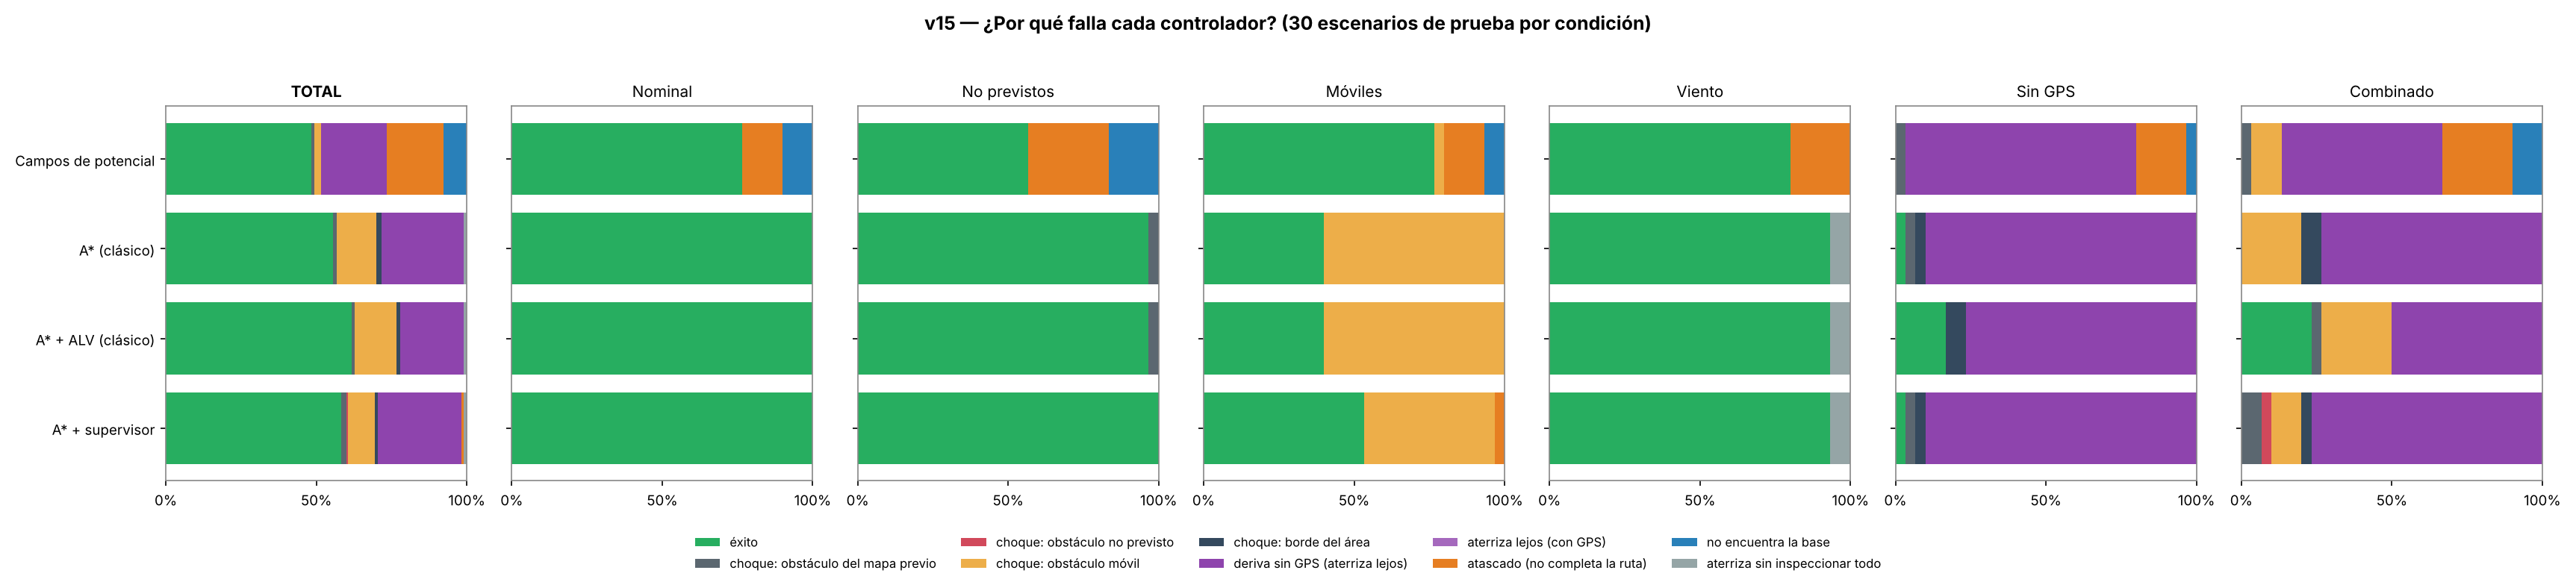
\includegraphics[width=0.95\textwidth]{v15_analisis_errores}
\caption{Causas de fallo por controlador y condición (\nfbEpisodiosPorCondicion{} escenarios
de prueba por condición).}
\label{fig:errores}
\end{figure*}

% Sección del artículo — dueño: P5. La tabla se genera desde results/v19_costo.csv.
\subsection{Costo computacional}
Todo el pipeline (datos, entrenamiento de las cuatro redes de la mosca, DAgger y la abeja con
tres semillas, benchmark, ablaciones e interpretabilidad) se ejecuta con un comando en Google
Colab (GPU \nfbGPU{}); consumió \nfbHorasGPU{} horas de GPU y \nfbHorasTotales{} horas en total
(Tabla~\ref{tab:costo}). Las redes son pequeñas (\nfbParamsGRU{} parámetros la mosca), por lo
que la inferencia tarda milisegundos por decisión en CPU, compatible con un computador de a
bordo; el simulador y las líneas base clásicas corren sin GPU.

\begin{table}[t]
\caption{Costo computacional por etapa (generado desde \texttt{v19\_costo.csv})}
\label{tab:costo}
\centering
\begin{tabular}{lrr}
\toprule
Etapa & Minutos & Horas de GPU \\
\midrule
\multicolumn{3}{c}{\pendiente{ejecutar scripts/run\_pipeline.py en Colab}} \\
\bottomrule
\end{tabular}
\end{table}


% Sección del artículo — dueño: P3.
\section{Discusión}\label{sec:discusion}
\textbf{Por qué funciona (o no).} Los métodos clásicos fallan por dos razones distintas que
el análisis de errores separa con claridad: planifican sobre un mapa que deja de ser cierto
cuando aparecen obstáculos móviles, y sin GPS confían en una posición estimada que deriva con
el viento. La división del trabajo inspirada en insectos ataca cada causa con un módulo
distinto: la memoria temporal de la mosca permite anticipar el movimiento a partir de varios
cuadros, y la abeja no estima \emph{dónde está} el dron sino \emph{hacia dónde está la base},
una señal que no acumula error. \pendiente{confirmar o refutar con los resultados de v19}

\textbf{Limitaciones.} Los datos son sintéticos: el movimiento es plano (2.5D) y los
sensores son abstracciones. El ojo de la mosca es un mapa de ocupación, no una imagen, y la
panorámica ignora iluminación, vegetación, texturas y la inclinación del dron por el viento,
que Bee-Nav~\cite{ou2026} identifica como la principal causa de fallo en exterior; además, la
elevación se mide desde el suelo y no desde la altura del dron. La validación del sensor
(Fig.~\ref{fig:sensor}) muestra que la silueta conserva las propiedades que necesita el
retorno visual, pero no sustituye una prueba con imágenes reales. Las redes publicadas de
retorno visual~\cite{firlefyn2024,ou2026} no se reentrenaron sobre nuestros datos, de modo que
la comparación con ellas es sólo de diseño y de tamaño, no de rendimiento. El experto es un
planificador con información privilegiada, así que la mosca hereda sus sesgos (por ejemplo,
su preferencia por ciertas maniobras). Las misiones son cortas (área de 60\,m) y no hay
modelo aerodinámico; el alcance de los rayos (8\,m) es mayor que el de sensores ToF
comerciales pequeños. Ninguna de estas conclusiones se ha validado todavía en un dron físico.

\textbf{Sesgos y riesgos de uso.} Los escenarios son procedurales: no representan una
geografía real ni su distribución de obstáculos. Un controlador que vuela sin GPS reduce la
supervisión humana; debe usarse con un piloto capaz de tomar el control, dentro de la
regulación de la autoridad aeronáutica y con respeto a la privacidad de las personas en las
zonas inspeccionadas. No debe usarse para vigilancia de personas.

\textbf{Impacto.} Si el resultado se sostiene con sensores reales, un dron de bajo costo
podría inspeccionar quebradas, puentes y canales cubiertos y volver sin GPS, con redes de
pocos cientos de miles de parámetros que caben en un computador de a bordo.

% Sección del artículo — dueño: P1.
\section{Conclusiones}
Presentamos NeuroFly-Bee, un controlador bioinspirado que separa el control local (mosca,
CNN+GRU) del retorno visual (abeja, red siamesa) y lo protege con un supervisor de seguridad.
En un simulador reproducible con seis condiciones, las líneas base clásicas completan como
máximo el \nfbMejorClasicoSinGPS{} de las misiones sin GPS y el \nfbMejorClasicoMoviles{} con
obstáculos móviles, y el análisis de errores atribuye esos fallos a la deriva y a planificar
sobre un mapa obsoleto. \pendiente{hallazgo principal del híbrido con los números de v19}

La validación del sensor muestra que la silueta 2.5D conserva las propiedades de los
panoramas reales que necesita el retorno visual, y la ablación en prueba mide cuánto aporta
comparar con la vista de casa: \nfbAblAbejaCompleta{} con ella frente a
\nfbAblAbejaVistaUnica{} sin ella.

Como trabajo futuro: (i) renderizar panoramas en 3D con dinámica de actitud, por ejemplo con
PyBullet~\cite{panerati2021}, aleatorizando texturas e iluminación~\cite{tobin2017};
(ii) evaluar la abeja sin reentrenar sobre las imágenes reales de bosque de Firlefyn
et~al.~\cite{firlefyn2024}, publicadas con licencia CC0, y reentrenar las arquitecturas de
Bee-Nav~\cite{ou2026} sobre nuestros datos para compararlas en igualdad de condiciones;
(iii) calibrar el viento con datos meteorológicos de cuencas peruanas y con el modelo de
turbulencia de Dryden; (iv) cuantizar las redes para un microcontrolador; y (v) validar el
sistema en un dron físico.

% Sección del artículo — dueño: P3 + todos. OBLIGATORIA (sin ella el artículo está incompleto).
% Nombres completos: los mismos (y en el mismo orden) que en 00_autores.tex.
% v24: tareas alineadas con lo implementado; cada integrante debe confirmar las suyas.
\section*{Contribuciones}
\noindent\begin{tabular}{@{}p{0.30\linewidth}p{0.66\linewidth}@{}}
\toprule
Integrante & Tareas en las que participó \\
\midrule
Nombre Apellido 1 & Propuesta y formulación del problema, simulador, sensores,
experto, líneas base, controlador híbrido, visor y simulación en vivo, contratos del
repositorio, introducción y conclusiones \\
Nombre Apellido 2 & Trabajos relacionados, interpretabilidad (Grad-CAM e Integrated
Gradients), validación del sensor panorámico 2.5D \\
Nombre Apellido 3 & Datos y particiones, edición del artículo, resumen, metodología de datos
y discusión \\
Nombre Apellido 4 & Benchmark, ablaciones (arquitecturas de la mosca, DAgger y red de la
abeja), significancia estadística, resultados y diapositivas \\
Nombre Apellido 5 & Entrenamiento en Colab y pipeline, DAgger, red de la abeja, AUROC, costo
computacional, cuaderno de demostración y arquitectura \\
\bottomrule
\end{tabular}

% Sección del artículo — dueño: P1.
\section*{Disponibilidad y uso de herramientas de IA}
El código, las configuraciones, los resultados y las instrucciones para regenerar cada tabla
y figura están en el repositorio \pendiente{enlace con la etiqueta v1.0-final}; los pesos
entrenados, con su manifiesto SHA-256, en \pendiente{enlace a Hugging Face o Drive}. Cada
número del texto se genera con \texttt{scripts/collect\_results.py} desde los archivos de
resultados. Se usó el asistente de IA Claude (Anthropic) para programar, depurar y revisar
la redacción; los diseños, experimentos y conclusiones son responsabilidad del equipo y todos
los resultados provienen de nuestras propias ejecuciones.


\IfFileExists{IEEEtran.bst}{\bibliographystyle{IEEEtran}}{\bibliographystyle{ieeetr}}   % IEEEtran en Overleaf/TeX Live completo
\bibliography{refs}

\end{document}
